% Options for packages loaded elsewhere
\PassOptionsToPackage{unicode}{hyperref}
\PassOptionsToPackage{hyphens}{url}
\PassOptionsToPackage{dvipsnames,svgnames,x11names}{xcolor}
\documentclass[
  10pt,
]{article}
\usepackage{xcolor}
\usepackage[margin=1in]{geometry}
\usepackage{amsmath,amssymb}
\setcounter{secnumdepth}{-\maxdimen} % remove section numbering
\usepackage{iftex}
\ifPDFTeX
  \usepackage[T1]{fontenc}
  \usepackage[utf8]{inputenc}
  \usepackage{textcomp} % provide euro and other symbols
\else % if luatex or xetex
  \usepackage{unicode-math} % this also loads fontspec
  \defaultfontfeatures{Scale=MatchLowercase}
  \defaultfontfeatures[\rmfamily]{Ligatures=TeX,Scale=1}
\fi
\usepackage{lmodern}
\ifPDFTeX\else
  % xetex/luatex font selection
\fi
% Use upquote if available, for straight quotes in verbatim environments
\IfFileExists{upquote.sty}{\usepackage{upquote}}{}
\IfFileExists{microtype.sty}{% use microtype if available
  \usepackage[]{microtype}
  \UseMicrotypeSet[protrusion]{basicmath} % disable protrusion for tt fonts
}{}
\makeatletter
\@ifundefined{KOMAClassName}{% if non-KOMA class
  \IfFileExists{parskip.sty}{%
    \usepackage{parskip}
  }{% else
    \setlength{\parindent}{0pt}
    \setlength{\parskip}{6pt plus 2pt minus 1pt}}
}{% if KOMA class
  \KOMAoptions{parskip=half}}
\makeatother
\usepackage{longtable,booktabs,array}
\newcounter{none} % for unnumbered tables
\usepackage{calc} % for calculating minipage widths
% Correct order of tables after \paragraph or \subparagraph
\usepackage{etoolbox}
\makeatletter
\patchcmd\longtable{\par}{\if@noskipsec\mbox{}\fi\par}{}{}
\makeatother
% Allow footnotes in longtable head/foot
\IfFileExists{footnotehyper.sty}{\usepackage{footnotehyper}}{\usepackage{footnote}}
\makesavenoteenv{longtable}
\usepackage{graphicx}
\makeatletter
\newsavebox\pandoc@box
\newcommand*\pandocbounded[1]{% scales image to fit in text height/width
  \sbox\pandoc@box{#1}%
  \Gscale@div\@tempa{\textheight}{\dimexpr\ht\pandoc@box+\dp\pandoc@box\relax}%
  \Gscale@div\@tempb{\linewidth}{\wd\pandoc@box}%
  \ifdim\@tempb\p@<\@tempa\p@\let\@tempa\@tempb\fi% select the smaller of both
  \ifdim\@tempa\p@<\p@\scalebox{\@tempa}{\usebox\pandoc@box}%
  \else\usebox{\pandoc@box}%
  \fi%
}
% Set default figure placement to htbp
\def\fps@figure{htbp}
\makeatother
\setlength{\emergencystretch}{3em} % prevent overfull lines
\providecommand{\tightlist}{%
  \setlength{\itemsep}{0pt}\setlength{\parskip}{0pt}}
\usepackage{etoolbox}
\AtBeginEnvironment{longtable}{\scriptsize}
\setlength{\tabcolsep}{3pt}
\usepackage{float}
\floatplacement{figure}{H}
\usepackage{xurl}
\Urlmuskip=0mu plus 1mu
\usepackage{bookmark}
\IfFileExists{xurl.sty}{\usepackage{xurl}}{} % add URL line breaks if available
\urlstyle{same}
\hypersetup{
  pdftitle={The 2026 NBA Draft Big Board: A Five-Stream Evidence Pipeline},
  pdfauthor={Autonomous AI Scouting Department (Claude)},
  colorlinks=true,
  linkcolor={blue},
  filecolor={Maroon},
  citecolor={Blue},
  urlcolor={blue},
  pdfcreator={LaTeX via pandoc}}

\title{The 2026 NBA Draft Big Board: A Five-Stream Evidence Pipeline}
\author{Autonomous AI Scouting Department (Claude)}
\date{June 10, 2026 (draft: June 23-24, 2026)}

\begin{document}
\maketitle

{
\setcounter{tocdepth}{3}
\tableofcontents
}
\newpage

\section{1. Abstract}\label{abstract}

This project builds a complete, self-contained evaluation of the 2026 NBA Draft
class from raw public data to a final 30-player big board and a fit-adjusted
mock draft. Five evidence streams were collected and integrated: (1) a
six-outlet consensus board covering 45 prospects (ESPN, The Ringer, Yahoo,
Tankathon, CBS, Bleacher Report); (2) a 1,309-player historical dataset of the
2000-2021 draft classes enriched with final-season college statistics; (3) a
suite of leave-one-draft-class-out (LODCO) validated models, a ridge VORP
regression on skill features that beats the pick-slot market baseline within the
first round (Spearman 0.256 vs 0.145, MAE 7.25 vs 8.14), a five-tier career
classifier, and a calibrated bust logistic (AUC 0.794, Brier 0.176); (4) a
weighted z-space kNN comps engine over 781 historical NCAA draftees producing
15-player cohorts with floor, median, and ceiling outcomes; and (5) frame-based
film study of the consensus top 20 (roughly 11,000 stills at 1 fps, with
explicit honesty rules about what stills cannot show). The headline call is
Cameron Boozer at No.~1 over consensus No.~1 AJ Dybantsa: Boozer is the model's
top prospect by a wide margin (0.70 All-Star probability, 0.006 bust
probability), owns the best comp cohort in the class (Love, Bosh, Bogut; 40\%
All-Star rate), and is the youngest top prospect with the best efficiency (65.3
TS\% on 29.9 usage). Other headline calls: Mikel Brown Jr.~falls from consensus
7.5 to 14 on production evidence, Ebuka Okorie rises from 20 to 11, and Jayden
Quaintance is held at 25 as a priced medical swing. Every number in this report
traces to files in the project repository.

\section{2. Introduction and Problem
Statement}\label{introduction-and-problem-statement}

The NBA draft is a prediction-under-uncertainty problem with unusually punishing
economics. A team converts one pick into one player whose career value spans
roughly -2 to +159 VORP in our 2000-2021 outcome data, with a heavily
right-skewed distribution: 43.6\% of all drafted players in that window meet a
``bust'' definition (under 100 career games or under 2 win shares), while a
handful of picks return franchise-altering value. The market's own signal, the
pick slot itself, explains only part of the variance (first-round Spearman of
0.145 against career VORP in our out-of-fold evaluation). Any single information
source, scouting consensus, box-score production, measurements, or film, is
individually weak; the practical question is how to combine them without letting
any one stream silently dominate.

This project treats the 2026 class as a full-stack research exercise and answers
with five deliberately separated evidence streams:

\begin{enumerate}
\def\labelenumi{\arabic{enumi}.}
\tightlist
\item
  \textbf{Market consensus}: a merged six-outlet board (45 players) capturing
  what the industry collectively believes, including its disagreements
  (per-player rank spreads up to 17 slots).
\item
  \textbf{Historical outcome modeling}: regression, tier classification, and
  bust models trained on 1,309 drafted players (2000-2021) with college
  production, age, and anthropometrics as features, validated by leaving out
  entire draft classes.
\item
  \textbf{Statistical comps}: nearest-neighbor cohorts in a weighted z-scored
  feature space, summarized as floor/median/ceiling VORP and empirical bust and
  All-Star rates.
\item
  \textbf{First-party film}: 1 fps frame studies of the top 20 prospects with
  strict rules about which claims stills can support, paired with cited human
  scouting.
\item
  \textbf{Measurements and context}: 2026 combine anthropometrics and athletic
  testing (78 players), prospect season statistics with injury flags (40
  players), and team-by-team needs for all 30 first-round slots.
\end{enumerate}

The board itself is a talent-only expected-value ranking; team fit is
deliberately quarantined in a separate mock draft so that the two questions
(``who is best?'' and ``who should team X take?'') never contaminate each other.

\section{3. Related Work}\label{related-work}

Public, stat-driven draft modeling has a long informal tradition:
consensus-aggregation approaches that average or rank-merge multiple outlet
boards to estimate market value, and college-production regressions that map
NCAA box-score and advanced statistics (typically age, BPM-family metrics,
usage, and efficiency) onto NBA career outcomes such as VORP, win shares, or
rotation survival. Published public models consistently find that age at draft
and overall college impact metrics carry most of the recoverable signal, that
draft slot itself is a strong baseline because it aggregates private team
intelligence, and that out-of-class validation is essential because outcomes
within a draft class are correlated. This project follows that general design
philosophy, market baseline first, skill models second, honest comparison
between them, without depending on any specific prior implementation; all
results here are derived from data collected in this repository.

\section{4. Data}\label{data}

All data were collected on June 10, 2026, from public sources, with raw
snapshots preserved under \texttt{data/raw/}. Full provenance is in
\texttt{sources.md}; per-dataset collection notes live in
\texttt{data/raw/*.md}.

\subsection{4.1 Dataset summary}\label{dataset-summary}

{\def\LTcaptype{none} % do not increment counter
\begin{longtable}[]{@{}
  >{\raggedright\arraybackslash}p{(\linewidth - 8\tabcolsep) * \real{0.0686}}
  >{\raggedright\arraybackslash}p{(\linewidth - 8\tabcolsep) * \real{0.1661}}
  >{\raggedright\arraybackslash}p{(\linewidth - 8\tabcolsep) * \real{0.1083}}
  >{\raggedright\arraybackslash}p{(\linewidth - 8\tabcolsep) * \real{0.3755}}
  >{\raggedright\arraybackslash}p{(\linewidth - 8\tabcolsep) * \real{0.2816}}@{}}
\toprule\noalign{}
\begin{minipage}[b]{\linewidth}\raggedright
Dataset
\end{minipage} & \begin{minipage}[b]{\linewidth}\raggedright
File
\end{minipage} & \begin{minipage}[b]{\linewidth}\raggedright
Size
\end{minipage} & \begin{minipage}[b]{\linewidth}\raggedright
Source / method
\end{minipage} & \begin{minipage}[b]{\linewidth}\raggedright
Known gaps
\end{minipage} \\
\midrule\noalign{}
\endhead
\bottomrule\noalign{}
\endlastfoot
Draft order 2026 & \texttt{data/processed/draft\_order.csv} & 30 picks &
Tankathon + CBS cross-validated; Wikipedia for trade provenance & Pick 22/30
routing details single-source, flagged UNVERIFIED \\
Consensus board & \texttt{data/processed/consensus\_board.csv} & 45 players, 6
outlets & ESPN, Ringer, Yahoo (KOC Mock 7.0), Tankathon, CBS, Bleacher Report &
Ringer truncated at 30; CBS at 28; NBADraft.net 403; The Athletic paywalled \\
Combine 2026 & \texttt{data/processed/combine\_2026.csv} & 78 rows (75 anthro,
71 tested) & Wayback snapshots of NBADraft.net tables, cross-checked vs Yahoo
and ESPN & Height-in-shoes, hand size, body fat blank for all (stats.nba.com
unreachable) \\
Prospect stats 2026 & \texttt{data/processed/prospect\_stats\_2026.csv} & 40
players, 29 cols & Sports-Reference per-player pages; RealGM for birthdates and
international stats & 3 internationals have UNVERIFIED usage/BPM (not published
for their leagues) \\
Historical outcomes & \texttt{data/processed/historical.csv} & 1,309 players,
2000-2021 & Basketball-Reference draft pages + player index; Wikipedia All-Star
list; GitHub combine-anthro snapshot & Wingspan 63\% coverage;
\textasciitilde12\% never played (outcomes are true zeros) \\
Historical enriched & \texttt{data/processed/historical\_enriched.csv} & 1,309
rows, 36 cols & + Barttorvik bulk data (2009-2021) and Sports-Reference college
pages (2000-2008 first-rounders) & Advanced rates 34\% pre-2009; internationals
blank by design \\
Comps & \texttt{data/processed/comps\_2026.csv} & 40 prospects &
\texttt{src/comps\_engine.py} over a 781-player NCAA pool & 3 internationals LOW
confidence \\
Model predictions & \texttt{models/predictions\_2026.csv} & 40 prospects &
\texttt{src/apply\_2026.py}, ridge + tier + bust models, 200-rep bootstrap & 5
consensus-board players not modeled (no stats row) \\
Film & \texttt{film/notes/} + \texttt{film/frames/} & 20 prospects,
\textasciitilde11,000 frames & yt-dlp 480p clips, ffmpeg 1 fps extraction &
Stills only; 2 prospects without clean jumper reps sampled \\
Team fit / mock & \texttt{data/processed/team\_fit.md}, \texttt{mock\_draft.csv}
& 30 slots / 30 picks & \texttt{team\_context.md} (24 team entries) +
project-internal files & Cap/apron details UNVERIFIED where no June 2026 source
found \\
\end{longtable}
}

\subsection{4.2 Consensus board}\label{consensus-board}

Six outlet boards were fetched on June 10, 2026 and merged by normalized player
name into \texttt{consensus\_board.csv} (45 players with per-outlet ranks plus
mean, median, min, max, and spread). Two boards are partially truncated (The
Ringer stops at pick 30, CBS at 28), so deep ranks average over fewer outlets.
The consensus top five: Dybantsa (median 1.0), Peterson (2.0), Boozer (3.0),
Wilson (4.0), Wagler (5.0). The market's internal disagreements are themselves
informative: Luigi Suigo's spread is 17 slots, Karim Lopez 16, Joshua Jefferson
13. NBADraft.net returned HTTP 403 and The Athletic is paywalled; both were
skipped and documented in \texttt{data/raw/consensus\_notes.md}.

\subsection{4.3 2026 combine}\label{combine}

The combine (May 10-17, 2026, Chicago) tables were recovered from Wayback
Machine snapshots of NBADraft.net (the live pages are Cloudflare-blocked) and
cross-validated against Yahoo's independent 73-row table and ESPN spot checks.
The file holds 78 player rows: 75 with anthro, 71 with athletic testing.
Height-in-shoes, hand length/width, and body fat are blank for every player:
those columns exist only on stats.nba.com, whose API timed out on every attempt
and has no Wayback snapshot, and no secondary outlet republished them
(\texttt{data/raw/combine\_notes.md}). Notable absences: Quaintance and Saunders
measured but skipped testing post-injury; Kayil and De Larrea were no-shows
(overseas club seasons still running). Source discrepancies (e.g., Dybantsa
wingspan 7'0.5'' vs 7'0.25'' across outlets) are logged with the resolution rule
used; two garbled search-snippet numbers (a vertical misattributed to Stirtz,
another to Cenac) were caught against the full tables and discarded.

\subsection{4.4 2026 prospect statistics}\label{prospect-statistics}

Forty prospects (the Tankathon top-40 list) have full 2025-26 season lines from
Sports-Reference (per-game plus advanced) and birthdates from RealGM, with 100\%
coverage on birthdate, TS\%, and BPM. The three internationals (Lopez, Suigo, De
Larrea) carry pro-league counting stats with usage/AST\%/BPM marked UNVERIFIED,
as those leagues do not publish them. Injury flags captured at collection:
Peterson hamstring (24 GP), Wilson broken thumb (24 GP), Brown back (21 GP),
Quaintance knee (4 GP), Saunders ACL (torn Feb 14, 2026, out).

\subsection{4.5 Historical dataset
(2000-2021)}\label{historical-dataset-2000-2021}

\texttt{src/build\_historical.py} parses 22 Basketball-Reference draft pages
(one transient 403, recovered with a single backoff) into 1,309 rows: every pick
in both rounds with career-to-date G, MP, WS, WS/48, BPM, VORP, plus drafting
team and college. Birthdates and listed height/weight come from the BBR player
index (5,416 rows); the All-Star flag from Wikipedia's all-time list (466
players, with name-collision logic); historical combine anthro from a public
GitHub snapshot of the stats.nba.com API (1,788 rows, combine seasons
2000-2025), since the live API was unreachable. Per
\texttt{data/raw/historical\_coverage.md}: age coverage 88\%, height/weight
92\%, wingspan and standing reach 63\% (59\% for 2000-2009 classes, 68\% for
2010-2019, 52\% for 2020-2021), career outcome columns 88\% (blank only for the
\textasciitilde12\% who never played an NBA game; in modeling these are filled
with true zeros, not imputations). Nothing was imputed at the data layer.

The enrichment pass (\texttt{src/enrich\_college\_stats.py}) adds
final-college-season statistics from two sources: Barttorvik bulk data for the
2009-2021 classes (61,061 player-season rows, spot-checked against public season
lines for Zion Williamson, Curry, Davis, Trae Young, and Hield, all matching)
and scraped Sports-Reference college pages for 2000-2008 first-round picks
(snapshots in \texttt{data/raw/historical/college/sref/}, match decisions in
\texttt{match\_log.md}). Coverage: 100\% of NCAA first-rounders 2009-2021,
98.5\% for 2000-2008; usage and advanced rates are thinner pre-2009 (34\%)
because the 2000-2008 scrape was scoped to first-rounders, a documented cut.
International draftees have blank NCAA columns by design. The result is
\texttt{historical\_enriched.csv} (1,309 rows, 36 columns).

Per-year row counts and feature coverage (\%), reproduced from
\texttt{data/raw/historical\_coverage.md}:

{\def\LTcaptype{none} % do not increment counter
\begin{longtable}[]{@{}
  >{\raggedright\arraybackslash}p{(\linewidth - 22\tabcolsep) * \real{0.0714}}
  >{\raggedright\arraybackslash}p{(\linewidth - 22\tabcolsep) * \real{0.0714}}
  >{\raggedright\arraybackslash}p{(\linewidth - 22\tabcolsep) * \real{0.0536}}
  >{\raggedright\arraybackslash}p{(\linewidth - 22\tabcolsep) * \real{0.1071}}
  >{\raggedright\arraybackslash}p{(\linewidth - 22\tabcolsep) * \real{0.1071}}
  >{\raggedright\arraybackslash}p{(\linewidth - 22\tabcolsep) * \real{0.1429}}
  >{\raggedright\arraybackslash}p{(\linewidth - 22\tabcolsep) * \real{0.0893}}
  >{\raggedright\arraybackslash}p{(\linewidth - 22\tabcolsep) * \real{0.0893}}
  >{\raggedright\arraybackslash}p{(\linewidth - 22\tabcolsep) * \real{0.0536}}
  >{\raggedright\arraybackslash}p{(\linewidth - 22\tabcolsep) * \real{0.0893}}
  >{\raggedright\arraybackslash}p{(\linewidth - 22\tabcolsep) * \real{0.0536}}
  >{\raggedright\arraybackslash}p{(\linewidth - 22\tabcolsep) * \real{0.0714}}@{}}
\toprule\noalign{}
\begin{minipage}[b]{\linewidth}\raggedright
year
\end{minipage} & \begin{minipage}[b]{\linewidth}\raggedright
rows
\end{minipage} & \begin{minipage}[b]{\linewidth}\raggedright
age
\end{minipage} & \begin{minipage}[b]{\linewidth}\raggedright
height
\end{minipage} & \begin{minipage}[b]{\linewidth}\raggedright
weight
\end{minipage} & \begin{minipage}[b]{\linewidth}\raggedright
wingspan
\end{minipage} & \begin{minipage}[b]{\linewidth}\raggedright
reach
\end{minipage} & \begin{minipage}[b]{\linewidth}\raggedright
games
\end{minipage} & \begin{minipage}[b]{\linewidth}\raggedright
WS
\end{minipage} & \begin{minipage}[b]{\linewidth}\raggedright
WS/48
\end{minipage} & \begin{minipage}[b]{\linewidth}\raggedright
BPM
\end{minipage} & \begin{minipage}[b]{\linewidth}\raggedright
VORP
\end{minipage} \\
\midrule\noalign{}
\endhead
\bottomrule\noalign{}
\endlastfoot
2000 & 58 & 86 & 93 & 93 & 41 & 41 & 86 & 86 & 86 & 86 & 86 \\
2001 & 57 & 86 & 91 & 91 & 70 & 70 & 86 & 86 & 86 & 86 & 86 \\
2002 & 57 & 84 & 95 & 95 & 67 & 67 & 84 & 84 & 84 & 84 & 84 \\
2003 & 58 & 81 & 83 & 83 & 50 & 50 & 81 & 81 & 81 & 81 & 81 \\
2004 & 59 & 78 & 90 & 90 & 61 & 61 & 78 & 78 & 78 & 78 & 78 \\
2005 & 60 & 92 & 92 & 92 & 63 & 63 & 92 & 92 & 92 & 92 & 92 \\
2006 & 60 & 87 & 88 & 88 & 50 & 50 & 87 & 87 & 87 & 87 & 87 \\
2007 & 60 & 82 & 92 & 92 & 65 & 65 & 82 & 82 & 80 & 80 & 82 \\
2008 & 60 & 85 & 97 & 97 & 55 & 55 & 85 & 85 & 85 & 85 & 85 \\
2009 & 60 & 83 & 87 & 87 & 70 & 70 & 83 & 83 & 83 & 83 & 83 \\
2010 & 60 & 85 & 90 & 90 & 73 & 73 & 85 & 85 & 85 & 85 & 85 \\
2011 & 60 & 90 & 92 & 92 & 70 & 70 & 90 & 90 & 90 & 90 & 90 \\
2012 & 60 & 93 & 95 & 95 & 83 & 83 & 93 & 93 & 93 & 93 & 93 \\
2013 & 60 & 85 & 88 & 88 & 70 & 68 & 85 & 85 & 85 & 85 & 85 \\
2014 & 60 & 90 & 95 & 95 & 70 & 70 & 90 & 90 & 90 & 90 & 90 \\
2015 & 60 & 73 & 80 & 80 & 58 & 58 & 73 & 73 & 73 & 73 & 73 \\
2016 & 60 & 92 & 93 & 93 & 62 & 62 & 92 & 92 & 92 & 92 & 92 \\
2017 & 60 & 95 & 95 & 95 & 63 & 63 & 95 & 95 & 95 & 95 & 95 \\
2018 & 60 & 95 & 98 & 98 & 63 & 63 & 95 & 95 & 95 & 95 & 95 \\
2019 & 60 & 97 & 98 & 98 & 68 & 68 & 97 & 97 & 97 & 97 & 97 \\
2020 & 60 & 97 & 97 & 97 & 40 & 40 & 97 & 97 & 97 & 97 & 97 \\
2021 & 60 & 93 & 95 & 95 & 63 & 63 & 93 & 93 & 93 & 93 & 93 \\
\end{longtable}
}

Wingspan coverage is the weak column throughout (combine-era artifact); career
outcome coverage tracks the never-played share of each class.

\subsection{4.6 Cleaning decisions and gaps,
summarized}\label{cleaning-decisions-and-gaps-summarized}

\begin{itemize}
\tightlist
\item
  height\_in mixes combine barefoot height with BBR listed height (387 flagged
  rows); 2026 prospects use listed height for consistency with the historical
  convention, with combine wingspan/reach/weight where measured.
\item
  Never-played players (161, notes column verifies ``never played'') have
  outcome columns set to 0 as real outcomes, not missing data.
\item
  2026 STL\% and BLK\% are not published for prospects and were approximated
  from per-game steals and blocks with fixed possession constants (formulas in
  \texttt{src/apply\_2026.py}); ordering is preserved, absolute level is
  approximate, and the choice is documented.
\item
  Five consensus-board players (Amari Allen, Maliq Brown, Jack Kayil, Braden
  Smith, Izaiyah Nelson) have no prospect-stats row and are not modeled.
\end{itemize}

\section{5. Methodology}\label{methodology}

\subsection{5.1 Consensus aggregation}\label{consensus-aggregation}

Each outlet board was extracted verbatim into
\texttt{data/raw/consensus\_notes.md}, then merged by normalized name
(\texttt{data/raw/build\_consensus.py}). Per player we report each outlet rank
plus mean, median, min, max, and spread. The median is the availability proxy
used downstream (team fit treats a player as plausibly available within roughly
+/-6 of his median). Truncated boards contribute only where they actually rank a
player; no rank is invented for missing entries.

\subsection{5.2 Model suite}\label{model-suite}

All models train on \texttt{historical\_enriched.csv} (n=1,309) with seed 42,
implemented in \texttt{src/model\_common.py} and \texttt{src/train\_models.py}.

\textbf{Baseline.} A pick-slot isotonic regression (monotone decreasing, fit per
training fold) is the market baseline. Archived multi-outlet boards do not exist
for 2000-2021, so draft slot serves as the market-consensus proxy; this is
standard practice and documented as such.

\textbf{Skill regression.} Ridge, lasso, and HistGradientBoosting on a
21-feature skill set: age at draft; height, weight, wingspan, standing reach,
wingspan-height differential; NCAA TS\%, USG\%, AST\%, TOV\%, STL\%, BLK\%,
FT\%, 3PA per 40 minutes, OBPM, BPM; and five explicit missingness indicators
(miss\_age, miss\_anthro, miss\_wingspan, miss\_ncaa\_core, miss\_ncaa\_adv).
Pick slot is excluded from skill models by design (we want the talent signal,
not the market echo); with-pick variants are reported for comparison only. The
target is career VORP under an asinh transform, chosen by a transform scan
(identity vs asinh vs signed-sqrt): raw VORP is extremely right-skewed (max 159
vs median 0), and asinh improved ridge MAE from 5.64 to 4.59 and pooled Spearman
by about 0.02 while handling negative VORP naturally. Metrics are always
computed back on the raw VORP scale. Missing features are median-imputed inside
each CV training fold; the indicators keep missingness explicit rather than
silent.

\textbf{Tier classifier.} A five-tier career outcome label predicted by
multinomial logistic regression and an HGB classifier on the same skill
features, against a pick-only logistic baseline. The tiers
(\texttt{models/tier\_definitions.md}, first match wins):

{\def\LTcaptype{none} % do not increment counter
\begin{longtable}[]{@{}llll@{}}
\toprule\noalign{}
Tier & Exact rule & n & Median career VORP \\
\midrule\noalign{}
\endhead
\bottomrule\noalign{}
\endlastfoot
AllStar & at least one All-Star selection & 119 & 21.0 \\
Starter & career minutes \textgreater= 12,000 and career WS \textgreater= 25 &
158 & 9.1 \\
Rotation & career minutes \textgreater= 5,000 and career WS \textgreater= 5 &
297 & 1.7 \\
Bench & career games \textgreater= 100 and career WS \textgreater{} 2 & 158 &
-0.2 \\
Bust & everything else & 577 & -0.1 \\
\end{longtable}
}

Tier medians are monotone in career VORP, which sanity-checks the ordering;
Bench and Bust separate on longevity rather than VORP, by design.

\textbf{Bust logistic.} Binary label
\texttt{bust\ =\ (career\_games\ \textless{}\ 100)\ OR\ (career\_ws\ \textless{}\ 2.0)},
base rate 43.6\% over all picks, 19.9\% among first-rounders, 11.0\% in the
lottery. The label deliberately does not depend on draft position, because the
skill models exclude pick.

\subsection{5.3 Validation: LODCO, and why random splits
leak}\label{validation-lodco-and-why-random-splits-leak}

All evaluation uses leave-one-draft-class-out cross-validation: 22 folds, each
holding out one full draft year (2000-2021). Random row-level splits leak in
this setting in two ways. First, outcomes within a class are correlated (shared
era, shared league context, a shared cap on available minutes and roles), so a
random split lets the model see the held-out class's context through its
classmates. Second, the deployment task is exactly a LODCO fold: ranking a class
the model has never seen. Reported metrics are out-of-fold predictions pooled
across all 22 folds, plus the mean of within-year Spearman (the within-class
ranking skill that matters on draft night). A known censoring caveat:
career-to-date outcomes give the 2020 and 2021 classes only 4-6 seasons of
accumulation, so those folds understate upside (2020-21 combined: 1 Starter, 10
All-Stars, 50 Busts out of 120); accepted per project design and documented in
\texttt{models/tier\_definitions.md}.

\subsection{5.4 Uncertainty: bootstrap over draft
classes}\label{uncertainty-bootstrap-over-draft-classes}

2026 predictions come with distributions, not points. The ridge model is refit
200 times on bootstrap resamples of the 22 draft classes (resampling whole
classes with replacement, seed 42). \texttt{pred\_vorp\_mean} is the mean of
bootstrap-only draws (model uncertainty); the percentile columns (p10 through
p90) additionally inject LODCO out-of-fold residual noise (sd 1.66 on the asinh
scale, estimated from picks 1-45) to describe outcome spread. Two distribution
corrections were required and are narrated in Section 7: a convexity fix
(inverse asinh is convex, so residual noise inflates means) and winsorization of
outcome draws at the historical maximum (159.4 VORP).

\subsection{5.5 Comps engine}\label{comps-engine}

\texttt{src/comps\_engine.py} (deterministic, no web access) computes weighted
z-scored distances over 15 features (heaviest weights: age 1.50; height, TS\%,
and usage 1.25 each) against a candidate pool of 781 NCAA draftees from the
enriched historical file. Missing features are handled by pairwise
renormalization: each pairwise distance averages only over features present for
both players, requiring at least 60\% of total feature weight to be shared, so a
missing wingspan shrinks the comparison set instead of silently zero-filling.
Outputs per prospect: the 5 nearest comps with their career VORP, and a
15-player cohort summarized as floor (25th percentile), median (50th), and
ceiling (90th percentile) cohort career VORP plus empirical bust and All-Star
rates (``cohort15''). International prospects (Lopez, De Larrea, Suigo) are
comped on a restricted anthro/age/basic-stats set and flagged LOW confidence.
Size or role mismatches inside a cohort are annotated (e.g., a creation-role
mismatch when AST\% differs wildly). Spot checks passed on the first iteration
(Boozer to Love/Bogut/Bosh; Mara to Hibbert/Mobley/Thabeet) and the v1 weights
shipped unchanged.

\subsection{5.6 Film protocol: stills-only honesty
rules}\label{film-protocol-stills-only-honesty-rules}

For each of the consensus top 20: a game or season highlight reel was located on
YouTube, downloaded with yt-dlp at 480p or below, and decomposed by ffmpeg into
1 fps stills (about 11,000 frames total). Notes
(\texttt{film/notes/\textless{}slug\textgreater{}.md}) follow a strict
two-section format: frame-based observations (ours, every claim tagged to
specific frame files) and sourced scouting observations (human scouts, cited
with URLs). The honesty rules: 1 fps stills can support claims about posture,
release height, body frame, positioning, and extension; they cannot support
claims about burst, speed, timing, or feel, and every note states explicitly
what is not claimed. Where no clean rep of a skill landed on a sampled second
(e.g., no jumper rep for Philon or Graves), no mechanics claim is made at all.
Three or four representative frames per top-10 prospect were copied to
\texttt{film/frames/\_report\_picks/}.

\subsection{5.7 Team fit and the board-vs-mock
separation}\label{team-fit-and-the-board-vs-mock-separation}

The big board ranks expected value per pick with zero fit input. Team fit lives
entirely in \texttt{team\_fit.md} (all 30 slots: pick provenance, needs,
timeline, best fits plausibly available, and an explicit fit-vs-talent verdict)
and \texttt{mock\_draft.csv} (a 30-pick simulation where players are available
within roughly +/-6 of consensus median and teams draft by need, tendency, and
value). This separation means a fit-driven reach (e.g., the Clippers taking
Ament at 5) appears in the mock with its reasoning, while the board remains a
pure talent ranking. The mock validated: 30 unique players, all availability
constraints satisfied.

\section{6. Model Results}\label{model-results}

\subsection{6.1 VORP regression: skill features beat the market
proxy}\label{vorp-regression-skill-features-beat-the-market-proxy}

All numbers are LODCO out-of-fold on the raw VORP scale, from
\texttt{models/metrics\_regression.json}.

The transform scan that selected the asinh target (ridge and HistGB, all picks):

{\def\LTcaptype{none} % do not increment counter
\begin{longtable}[]{@{}
  >{\raggedright\arraybackslash}p{(\linewidth - 8\tabcolsep) * \real{0.1429}}
  >{\raggedright\arraybackslash}p{(\linewidth - 8\tabcolsep) * \real{0.1169}}
  >{\raggedright\arraybackslash}p{(\linewidth - 8\tabcolsep) * \real{0.2987}}
  >{\raggedright\arraybackslash}p{(\linewidth - 8\tabcolsep) * \real{0.1299}}
  >{\raggedright\arraybackslash}p{(\linewidth - 8\tabcolsep) * \real{0.3117}}@{}}
\toprule\noalign{}
\begin{minipage}[b]{\linewidth}\raggedright
Transform
\end{minipage} & \begin{minipage}[b]{\linewidth}\raggedright
Ridge MAE
\end{minipage} & \begin{minipage}[b]{\linewidth}\raggedright
Ridge Spearman (pooled)
\end{minipage} & \begin{minipage}[b]{\linewidth}\raggedright
HistGB MAE
\end{minipage} & \begin{minipage}[b]{\linewidth}\raggedright
HistGB Spearman (pooled)
\end{minipage} \\
\midrule\noalign{}
\endhead
\bottomrule\noalign{}
\endlastfoot
identity & 5.64 & 0.255 & 5.65 & 0.210 \\
asinh & \textbf{4.59} & \textbf{0.273} & 4.59 & 0.249 \\
signed sqrt & 4.57 & 0.273 & 4.61 & 0.247 \\
\end{longtable}
}

Main comparison, all picks (n=1,309):

{\def\LTcaptype{none} % do not increment counter
\begin{longtable}[]{@{}
  >{\raggedright\arraybackslash}p{(\linewidth - 8\tabcolsep) * \real{0.3375}}
  >{\raggedright\arraybackslash}p{(\linewidth - 8\tabcolsep) * \real{0.0500}}
  >{\raggedright\arraybackslash}p{(\linewidth - 8\tabcolsep) * \real{0.0625}}
  >{\raggedright\arraybackslash}p{(\linewidth - 8\tabcolsep) * \real{0.2125}}
  >{\raggedright\arraybackslash}p{(\linewidth - 8\tabcolsep) * \real{0.3375}}@{}}
\toprule\noalign{}
\begin{minipage}[b]{\linewidth}\raggedright
Model
\end{minipage} & \begin{minipage}[b]{\linewidth}\raggedright
MAE
\end{minipage} & \begin{minipage}[b]{\linewidth}\raggedright
RMSE
\end{minipage} & \begin{minipage}[b]{\linewidth}\raggedright
Spearman (pooled)
\end{minipage} & \begin{minipage}[b]{\linewidth}\raggedright
Spearman (within-year mean)
\end{minipage} \\
\midrule\noalign{}
\endhead
\bottomrule\noalign{}
\endlastfoot
Pick-slot isotonic baseline & 5.26 & 10.21 & 0.208 & 0.245 \\
Ridge (skill) & 4.59 & 11.04 & 0.273 & 0.269 \\
Lasso (skill) & 4.59 & 11.09 & 0.274 & 0.277 \\
HistGB (skill) & 4.59 & 10.91 & 0.249 & 0.246 \\
Ridge (skill + pick) & 4.55 & 10.99 & 0.288 & 0.287 \\
HistGB (skill + pick) & 4.53 & 10.65 & 0.277 & 0.281 \\
\end{longtable}
}

First round only (picks 1-30, n=658, the 2026 use case):

{\def\LTcaptype{none} % do not increment counter
\begin{longtable}[]{@{}llll@{}}
\toprule\noalign{}
Model & MAE & Spearman (pooled) & Spearman (within-year mean) \\
\midrule\noalign{}
\endhead
\bottomrule\noalign{}
\endlastfoot
Pick-slot isotonic baseline & 8.14 & 0.145 & 0.211 \\
Ridge (skill) & 7.25 & \textbf{0.256} & 0.245 \\
Lasso (skill) & 7.26 & 0.246 & 0.245 \\
HistGB (skill) & 7.25 & 0.213 & 0.197 \\
Ridge (skill + pick) & 7.24 & 0.275 & 0.268 \\
HistGB (skill + pick) & 7.20 & 0.268 & 0.260 \\
\end{longtable}
}

Findings, stated plainly. Skill-only linear models beat the pick baseline on
every regression metric except RMSE (the transform deliberately stops chasing
the extreme right tail, which costs RMSE and is the right trade for ranking
prospects). Within the first round the gap is large in relative terms: Spearman
0.256 vs 0.145. Adding pick on top of skills helps a little more (0.288 pooled),
meaning the market does know things box scores do not (intel, film, character),
but the increment is small (about 0.015): most of the market's ranking
information is recoverable from age, NCAA stats, and anthro. Lasso and ridge are
a statistical tie; ridge was chosen for the 2026 application because it wins the
first-round subset and its coefficients are stable, while lasso confirms feature
selection (it zeroes 6 of 21 features and keeps the same leaders). HistGB
underperforms the linear models, an honest negative result discussed in Section
7.

\subsection{6.2 Tier classifier}\label{tier-classifier}

From \texttt{models/metrics\_tiers.json} (5 tiers, LODCO):

{\def\LTcaptype{none} % do not increment counter
\begin{longtable}[]{@{}lll@{}}
\toprule\noalign{}
Model & Accuracy & Macro-F1 \\
\midrule\noalign{}
\endhead
\bottomrule\noalign{}
\endlastfoot
Pick-only logistic baseline & 0.494 & 0.222 \\
Multinomial logistic (skill) & 0.466 & 0.266 \\
HGB classifier (skill) & 0.441 & 0.294 \\
\end{longtable}
}

The pick baseline wins raw accuracy by predicting only the dominant classes (its
confusion matrix never predicts AllStar, Starter, or Bench at all); the skill
models win macro-F1 by actually discriminating the rare tiers. Neither is
strong: five-way career-tier prediction from pre-draft statistics is hard, and
we say so. The multinomial logistic supplies the 2026 tier probabilities (better
calibrated than HGB, whose macro-F1 edge comes mostly from the Bench tier).

\subsection{6.3 Bust model: the pick baseline wins AUC, and we say
so}\label{bust-model-the-pick-baseline-wins-auc-and-we-say-so}

From \texttt{models/metrics\_bust.json}:

{\def\LTcaptype{none} % do not increment counter
\begin{longtable}[]{@{}lllll@{}}
\toprule\noalign{}
Model & AUC & Brier & Log loss & AUC (first round) \\
\midrule\noalign{}
\endhead
\bottomrule\noalign{}
\endlastfoot
Pick-only logistic baseline & \textbf{0.806} & 0.178 & 0.532 & \textbf{0.668} \\
Logistic (skill) & 0.794 & \textbf{0.176} & \textbf{0.516} & 0.642 \\
HGB (skill) & 0.776 & 0.184 & 0.539 & - \\
\end{longtable}
}

The pick baseline beats the skill model on bust AUC, both overall (0.806 vs
0.794) and within the first round (0.668 vs 0.642). Where a player gets picked
is genuinely the single best washout predictor, because the market aggregates
private intelligence we do not have. The skill logistic remains the production
bust model for two reasons: it is the only model that can actually be applied to
2026 prospects (who have no pick yet), and it is well calibrated (near-diagonal
reliability curve, Brier 0.176, slight underconfidence below p=0.3). The correct
reading of every 2026 \texttt{bust\_prob} is therefore ``skills-only risk,'' not
market-informed risk.

\subsection{6.4 Feature importance}\label{feature-importance}

\begin{figure}
\centering
\pandocbounded{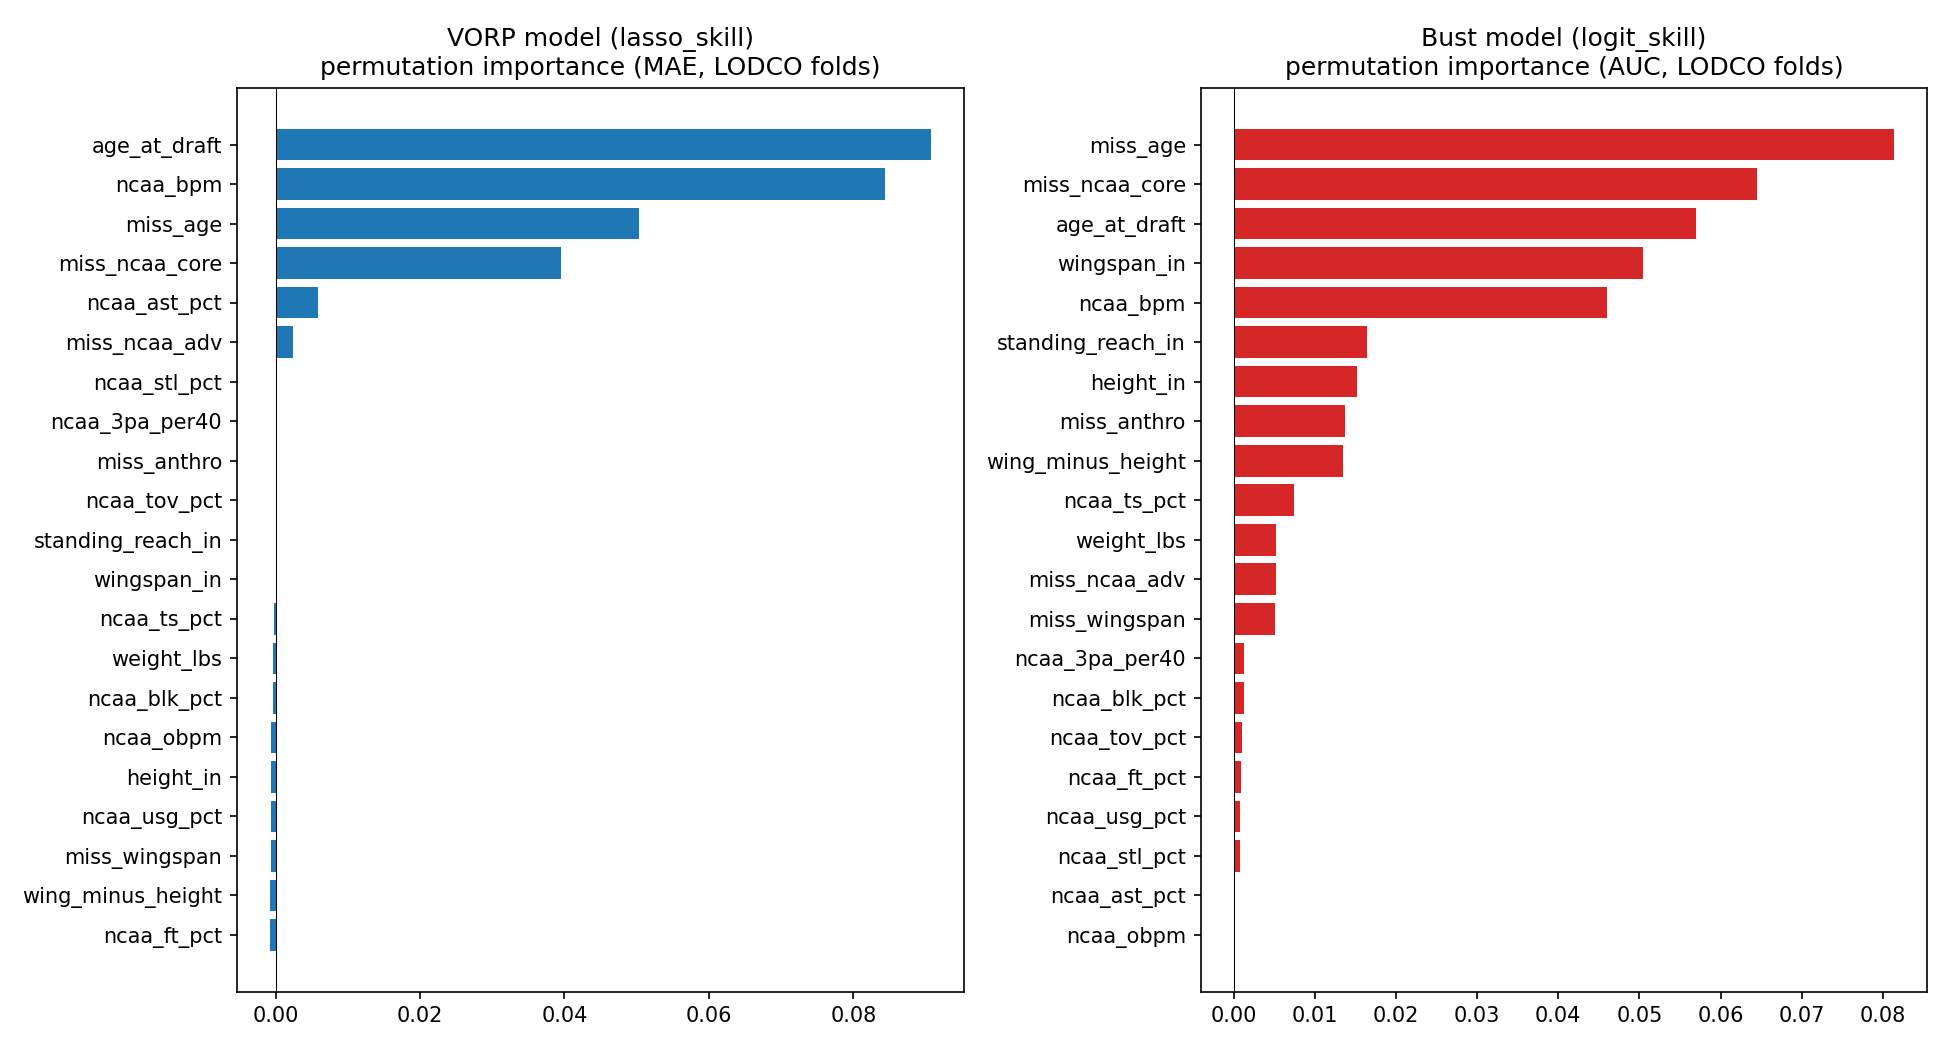
\includegraphics[keepaspectratio,alt={Permutation importance (LODCO test folds, 5 repeats per fold) for the VORP model. Age at draft and college BPM dominate; the missingness indicators carry real signal.}]{../figures/feature_importance.png}}
\caption{Permutation importance (LODCO test folds, 5 repeats per fold) for the
VORP model. Age at draft and college BPM dominate; the missingness indicators
carry real signal.}
\end{figure}

Top VORP-model features by permutation importance (standardized ridge
coefficients in parentheses): age\_at\_draft 0.091 (-0.38), ncaa\_bpm 0.084
(+0.35), miss\_age 0.050 (-0.17), miss\_ncaa\_core 0.039 (-0.24), ncaa\_ast\_pct
0.006 (+0.10). The hierarchy is clean: younger at the same production level is
far better; overall college impact is the second pillar; passing (AST\%) is the
clearest skill predictor after age and BPM; efficiency (TS\%, coef +0.05) and
free-throw touch (+0.03) help. Notable secondary findings: OBPM gets a negative
coefficient conditional on total BPM (given equal impact, defense-leaning
college players age better than offense-leaning ones, and lasso keeps the sign);
wingspan and reach contribute almost nothing to VORP once height and weight are
in (partly an artifact of 37\% wingspan missingness), yet wingspan is the No.~4
feature in the bust model; raw height is slightly negative conditional on
everything else (the skill stats already encode position, so raw ``big'' is not
a bonus). The bust model's top features are miss\_age, miss\_ncaa\_core,
age\_at\_draft, wingspan\_in, and ncaa\_bpm: older, statless, and short-armed is
the washout profile. A reading note for 2026 outputs: every NCAA prospect has
miss\_age = miss\_ncaa\_core = 0, so their scores ride on age, BPM, and AST\%;
the three internationals receive the miss\_ncaa\_core penalty, which functions
as the intended wide-uncertainty flag.

\begin{figure}
\centering
\pandocbounded{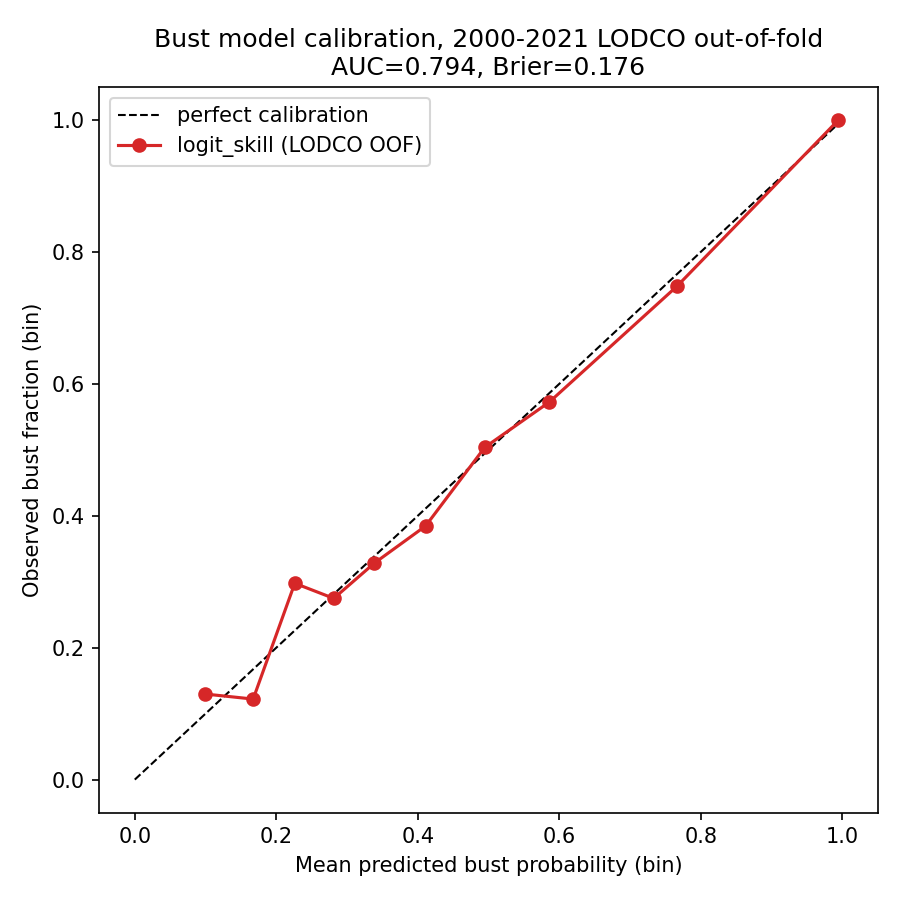
\includegraphics[keepaspectratio,alt={Reliability curve for the skill bust logistic (LODCO out-of-fold). Near-diagonal with slight underconfidence below p=0.3; Brier 0.176.}]{../figures/calibration_bust.png}}
\caption{Reliability curve for the skill bust logistic (LODCO out-of-fold).
Near-diagonal with slight underconfidence below p=0.3; Brier 0.176.}
\end{figure}

\subsection{6.5 Model vs consensus on the 2026
class}\label{model-vs-consensus-on-the-2026-class}

\begin{figure}
\centering
\pandocbounded{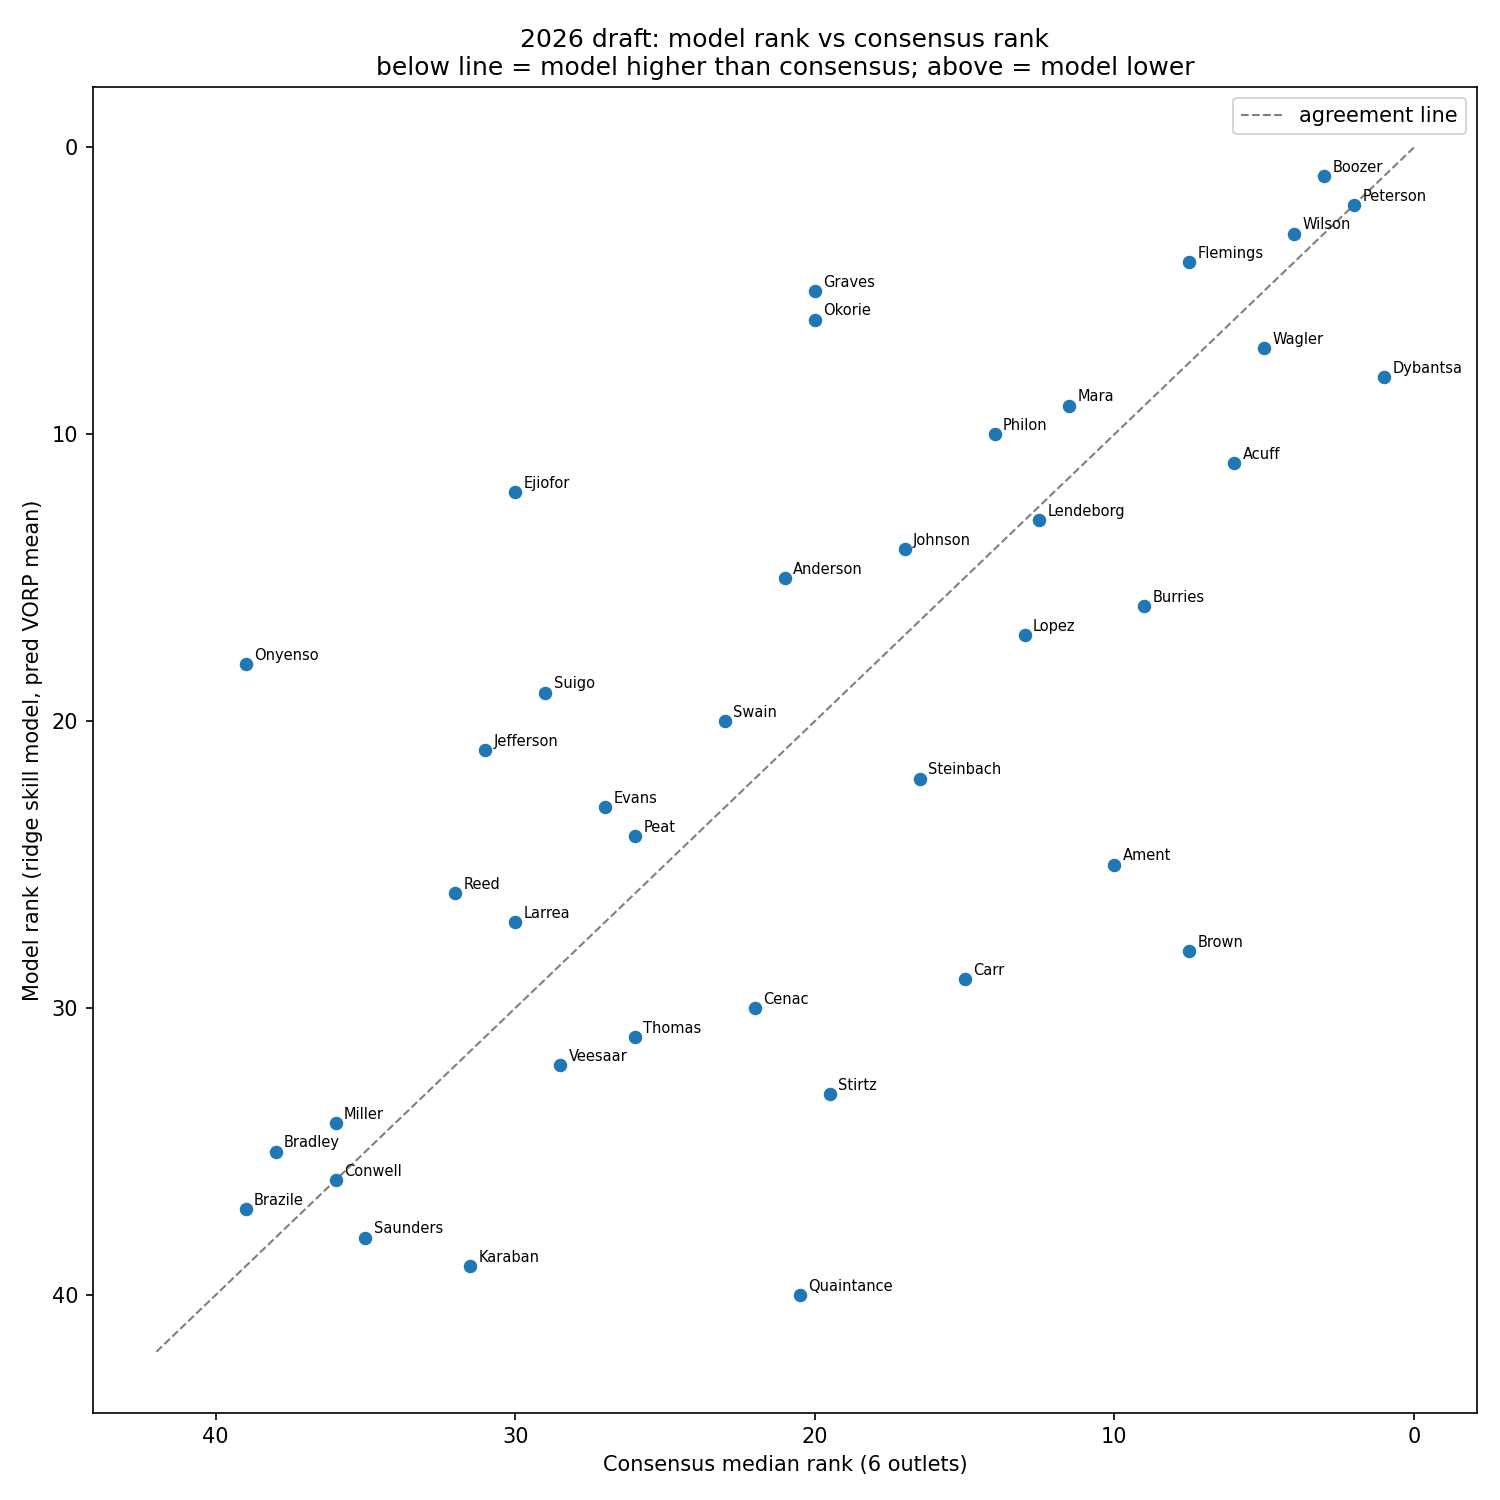
\includegraphics[keepaspectratio,alt={Model rank vs consensus median rank for the 40 modeled 2026 prospects. Points far off the diagonal are the disagreements analyzed in Sections 9 and 11.}]{../figures/pred_vs_consensus.png}}
\caption{Model rank vs consensus median rank for the 40 modeled 2026 prospects.
Points far off the diagonal are the disagreements analyzed in Sections 9 and
11.}
\end{figure}

The biggest gaps (consensus median minus model rank): model HIGHER on Onyenso
(+21), Ejiofor (+18), Graves (+15), Okorie (+14); model LOWER on Mikel Brown
(-20.5), Quaintance (-19.5), Ament (-15), Carr (-14), Stirtz (-13.5). The
pattern and its interpretation are taken up in Section 11.

\section{7. Iteration Narrative}\label{iteration-narrative}

Condensed from \texttt{models/iterations.md}; all runs
\texttt{python3\ src/train\_models.py}, seed 42 everywhere.

\textbf{Iteration 1, baseline and transform scan.} Established the pick-slot
isotonic baseline, then scanned target transforms. The asinh transform was
chosen: it lifted ridge from MAE 5.64 / pooled Spearman 0.255 to 4.59 / 0.273
(signed-sqrt essentially tied; asinh handles negative VORP without a sign hack).
RMSE got slightly worse under the transform because the model stops chasing the
Jokic/LeBron tail; accepted deliberately.

\textbf{Iteration 2, full model set.} The headline comparison of Section 6. Two
honest negative results landed here. First, HistGB underperforms ridge and lasso
(pooled Spearman 0.249 vs 0.273): with roughly 20 mostly linear features and
n=1.3k, trees add variance, not signal, so linear models are the headline
models. Second, the pick baseline beats the skill bust model on AUC (0.806 vs
0.794); documented rather than buried.

\textbf{Iteration 3, first-round-only training.} Since the 2026 board is a
top-45 exercise, we tested training only on picks 1-30 (n=658). It hurts:
FR-only ridge scores 0.235 pooled Spearman on first-rounders vs 0.256 for the
all-picks model evaluated on the same subset, and HGB collapses to 0.150.
Second-rounders roughly double n and sharpen the age and BPM gradients.
All-picks training kept.

\textbf{Iteration 4, 2026 application.} Refit ridge on all 22 classes, merged
the three 2026 files by normalized name (40 of 40 matched), and generated
bootstrap distributions. Two distribution bugs were caught and fixed, both
documented in code. (1) Convexity inflation: the first run reported the mean of
residual-noised draws; inverse asinh is convex, so the noise inflated means,
producing a nonsense 104 expected VORP for Boozer. Fix: report the mean of
bootstrap-only draws; keep residual noise only in the percentile columns, which
are meant to describe outcome spread. (2) Impossible tails: multiplicative
residual noise on the asinh scale let elite profiles draw outcomes above
anything in NBA history (p90 near 288 VORP, above LeBron's 159). Outcome draws
are clipped at the training maximum (159.4), affecting only the extreme right
tail of the top \textasciitilde3 prospects. Sanity checks passed: Boozer's
predicted mean of 22.4 VORP matches the historical average outcome of a No.~1
pick; the bust probability range (0.006 to 0.545) tops out on Quaintance (4 GP,
knee) and Mikel Brown, which is sensible; tier probabilities sum to 1.

The cross-cutting lesson: every fancier move was tested against a dumber
alternative, and three of them (gradient boosting, first-round-only training,
naively residual-noised means) lost or broke. What survived is a ridge
regression on 21 features, which is the point: the value is in the validation
design and the data, not in model exotica.

\section{8. Film Study}\label{film-study}

\subsection{8.1 Protocol}\label{protocol}

For each consensus top-20 prospect: locate a representative highlight reel or
single-game video, download at 480p or lower with yt-dlp, extract stills at 1
fps with ffmpeg, then write a two-section note: frame-based observations (every
claim tagged to specific frame files) and sourced scouting observations (cited
human scouts). Roughly 11,000 frames were extracted across the 20 prospects.
Video IDs and frame counts are recorded at the top of each note; clips are
preserved in \texttt{film/clips/}.

\subsection{8.2 What stills can and cannot
support}\label{what-stills-can-and-cannot-support}

Stills at 1 fps reliably show: release point and apex height relative to
contests, follow-through position, body frame relative to opponents in the same
frame, handle and post posture, base width, floor positioning, and extension at
the rim. They categorically cannot show: burst, first-step speed,
gather-to-release time, defensive timing, recovery quickness, or feel, because
the actual movement falls between sampled seconds. Every note carries an
explicit ``not claimed from frames'' list, and the highlight-reel sourcing adds
a made-plays-only selection bias that the notes also flag.

\subsection{8.3 Example observations}\label{example-observations}

\textbf{Cameron Boozer} (685 frames, ACC Digital Network reel,
\texttt{film/notes/boozer.md}). A post-up versus Texas Tech shows a wide, low
post seal with the defender pinned on his hip (frame\_0287 through frame\_0290),
then airborne at the rim a frame later with the ball carried high and away from
the swipe; the frames support a strong wide-base seal and high ball position,
not how quickly he elevated. Across multiple games he reads as already filled
out, thick through the chest, glutes, and thighs, holding base width under
contact. The reel produced no clean perimeter jumper rep at sampled seconds, so
the note makes no claim about his three-point set point.

\textbf{AJ Dybantsa} (1,503 frames, Big 12 Studios reel,
\texttt{film/notes/dybantsa.md}). A left-wing jumper versus Abilene Christian
(frame\_0544, ball flight at frame\_0547) releases above and slightly in front
of his head at the top of the jump, well above the closest defender's contest. A
finishing sequence versus California Baptist (frame\_0302 to frame\_0304) ends
fully extended at the rim with the ball above the cylinder, long and balanced
rather than crashing sideways. Close-ups show broad square shoulders on a lean
torso, a wing build with room for mass; nothing in the frames supports claims
about his famous burst, and the note says so.

\textbf{Aday Mara} (248 frames, Final Four versus Arizona,
\texttt{film/notes/mara.md}). Standing flat-footed under the basket his head
sits roughly at the bottom edge of the backboard (frame\_0061), so his set point
on any close shot starts above typical contest height before he leaves the
floor. He catches at the elbow with the ball kept at chest-to-chin level, torso
upright, shielding with the off shoulder rather than lowering into a dribble
crouch (frame\_0091, frame\_0181). Block timing and foot speed are explicitly
not claimable from stills.

\subsection{8.4 Selected report frames}\label{selected-report-frames}

\begin{figure}
\centering
\pandocbounded{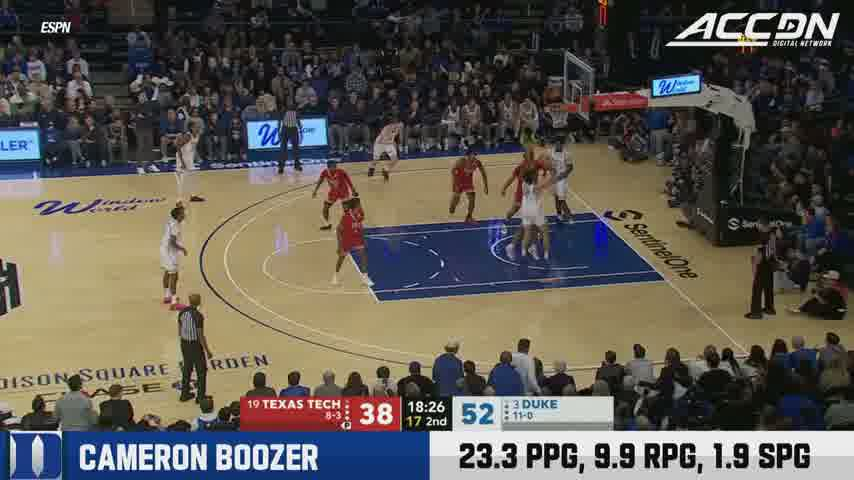
\includegraphics[keepaspectratio,alt={Cameron Boozer establishes a wide, low post seal on the right block vs Texas Tech, defender pinned on his hip (frame 0289).}]{../film/frames/_report_picks/boozer_pick1.jpg}}
\caption{Cameron Boozer establishes a wide, low post seal on the right block vs
Texas Tech, defender pinned on his hip (frame 0289).}
\end{figure}

\begin{figure}
\centering
\pandocbounded{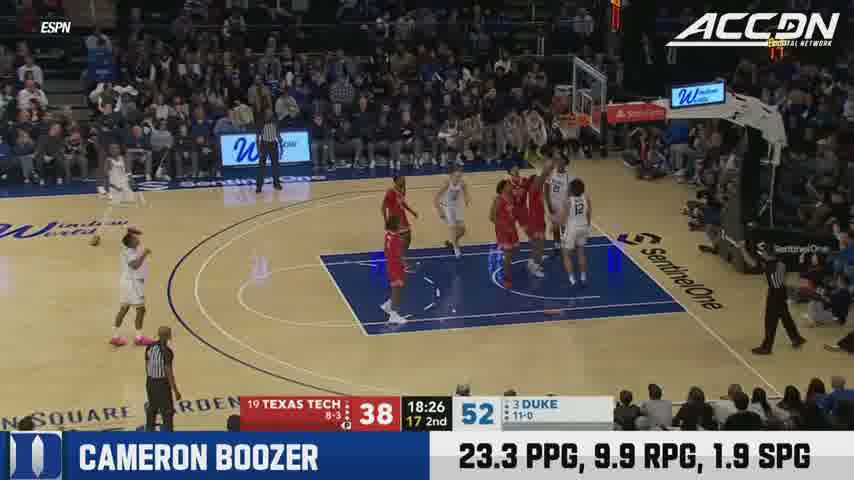
\includegraphics[keepaspectratio,alt={Cameron Boozer one frame later: airborne at the rim with the ball carried high and away from the swiping defender (frame 0290).}]{../film/frames/_report_picks/boozer_pick2.jpg}}
\caption{Cameron Boozer one frame later: airborne at the rim with the ball
carried high and away from the swiping defender (frame 0290).}
\end{figure}

\begin{figure}
\centering
\pandocbounded{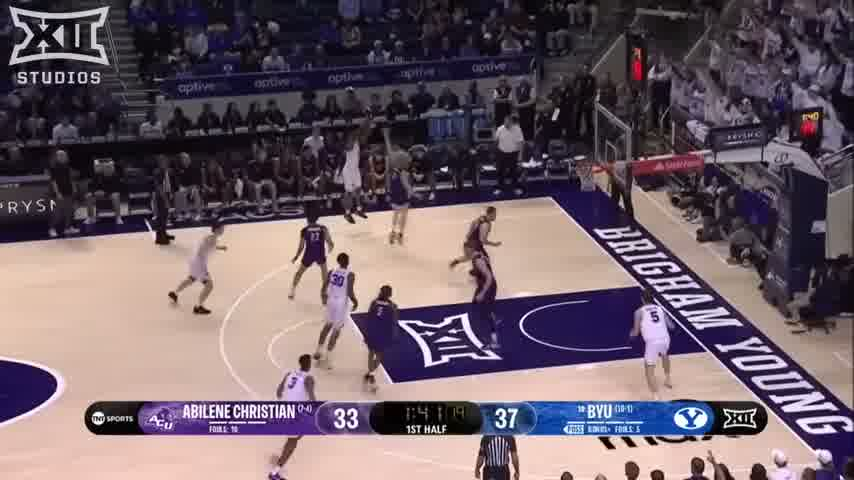
\includegraphics[keepaspectratio,alt={AJ Dybantsa at full elevation on a wing jumper, release point above the defender's contest (frame 0544).}]{../film/frames/_report_picks/dybantsa_pick1.jpg}}
\caption{AJ Dybantsa at full elevation on a wing jumper, release point above the
defender's contest (frame 0544).}
\end{figure}

\begin{figure}
\centering
\pandocbounded{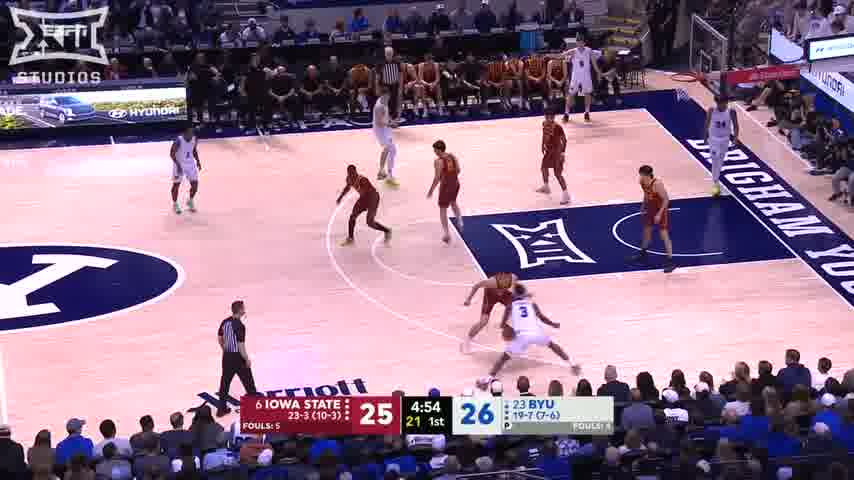
\includegraphics[keepaspectratio,alt={AJ Dybantsa in a low crouched handle posture attacking Iowa State, ball on his right hip, shoulders over knees (frame 1200).}]{../film/frames/_report_picks/dybantsa_pick4.jpg}}
\caption{AJ Dybantsa in a low crouched handle posture attacking Iowa State, ball
on his right hip, shoulders over knees (frame 1200).}
\end{figure}

\begin{figure}
\centering
\pandocbounded{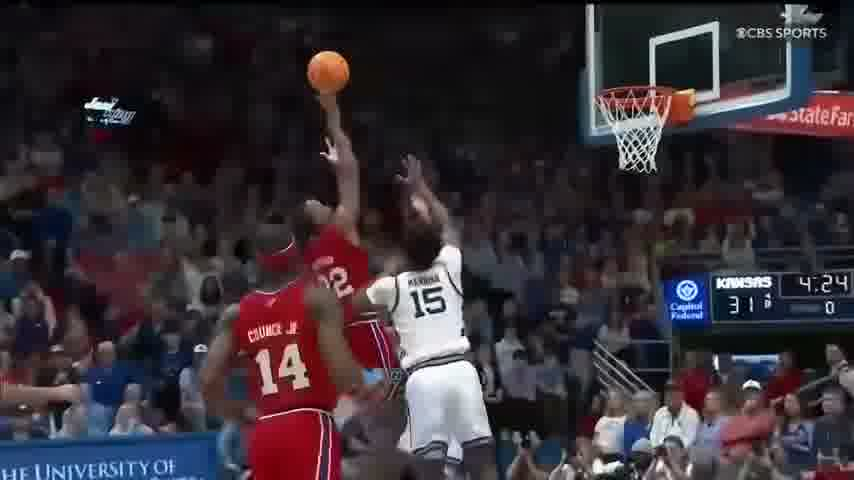
\includegraphics[keepaspectratio,alt={Darryn Peterson rises into a pull-up vs Kansas State with the ball above the contesting big's reach, balanced vertical body line at the apex (frame 0060).}]{../film/frames/_report_picks/peterson_pick2.jpg}}
\caption{Darryn Peterson rises into a pull-up vs Kansas State with the ball
above the contesting big's reach, balanced vertical body line at the apex (frame
0060).}
\end{figure}

\begin{figure}
\centering
\pandocbounded{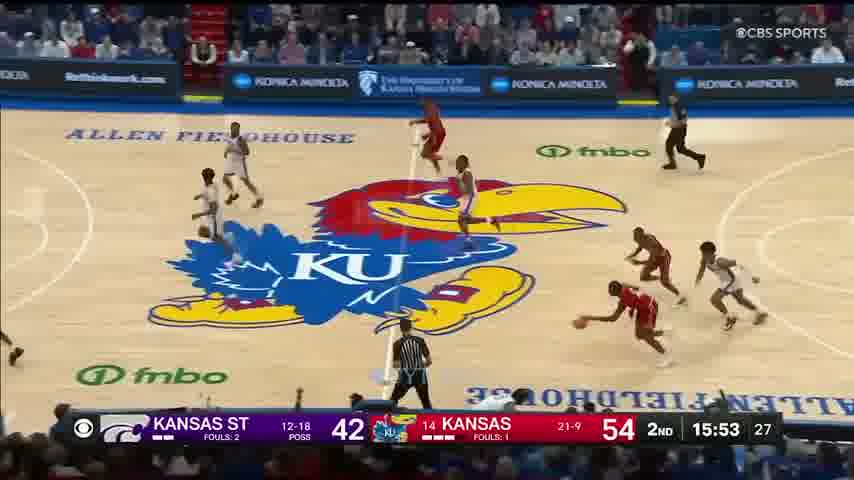
\includegraphics[keepaspectratio,alt={Darryn Peterson holds a high follow-through after an elbow jumper, arm fully extended, elbow above eye level (frame 0121).}]{../film/frames/_report_picks/peterson_pick4.jpg}}
\caption{Darryn Peterson holds a high follow-through after an elbow jumper, arm
fully extended, elbow above eye level (frame 0121).}
\end{figure}

\subsection{8.5 Limitations of the film
stream}\label{limitations-of-the-film-stream}

This is the weakest of the five evidence streams and is weighted accordingly.
The sampling rate destroys all motion information; the source reels are
made-play compilations with severe selection bias; several prospects are
represented by a single game; two prospects (Philon, Graves) produced no clean
jumper rep at sampled seconds despite shooting being central to their
evaluation, so their notes make no mechanics claims; Philon's only available
reel predates the sophomore leap his ranking depends on; one source (Burries)
was 360p. Player identification in wide frames sometimes rests on the reel being
that player's compilation rather than a legible jersey number, and the notes
flag this. The film stream is used to confirm or deny physical and postural
claims from scouting reports, never to generate athleticism or skill claims of
its own.

\section{9. The 2026 Big Board}\label{the-2026-big-board}

The board is a talent-only expected-value ranking built from all five evidence
streams (full per-player dossiers in \texttt{dossiers/}, assembled board in
\texttt{big\_board.md}, machine-readable ranking with per-player delta
rationales in \texttt{data/processed/final\_board.csv}).

\subsection{9.1 Tier definitions}\label{tier-definitions}

{\def\LTcaptype{none} % do not increment counter
\begin{longtable}[]{@{}
  >{\raggedright\arraybackslash}p{(\linewidth - 6\tabcolsep) * \real{0.0357}}
  >{\raggedright\arraybackslash}p{(\linewidth - 6\tabcolsep) * \real{0.0446}}
  >{\raggedright\arraybackslash}p{(\linewidth - 6\tabcolsep) * \real{0.2768}}
  >{\raggedright\arraybackslash}p{(\linewidth - 6\tabcolsep) * \real{0.6429}}@{}}
\toprule\noalign{}
\begin{minipage}[b]{\linewidth}\raggedright
Tier
\end{minipage} & \begin{minipage}[b]{\linewidth}\raggedright
Ranks
\end{minipage} & \begin{minipage}[b]{\linewidth}\raggedright
Label
\end{minipage} & \begin{minipage}[b]{\linewidth}\raggedright
Meaning
\end{minipage} \\
\midrule\noalign{}
\endhead
\bottomrule\noalign{}
\endlastfoot
1 & 1-4 & Franchise Cornerstones & Evidence (production, age, cohort) or ceiling
strong enough to build around \\
2 & 5-11 & High-Leverage Starters & Starter-probable profiles, several with live
star tails \\
3 & 12-18 & Starter-or-Bust Swings & Real starter cases with a documented flaw,
injury, or data gap on the other side \\
4 & 19-28 & Rotation Bets with Upside Tails & Likely rotation players whose
cohorts carry one famous tail outcome \\
5 & 29-30 & Specialists / Projects & One elite NBA skill or one defining fit,
priced at the end of the round \\
\end{longtable}
}

\subsection{9.2 The board at a glance}\label{the-board-at-a-glance}

{\def\LTcaptype{none} % do not increment counter
\begin{longtable}[]{@{}
  >{\raggedright\arraybackslash}p{(\linewidth - 14\tabcolsep) * \real{0.0488}}
  >{\raggedright\arraybackslash}p{(\linewidth - 14\tabcolsep) * \real{0.2195}}
  >{\raggedright\arraybackslash}p{(\linewidth - 14\tabcolsep) * \real{0.0610}}
  >{\raggedright\arraybackslash}p{(\linewidth - 14\tabcolsep) * \real{0.2439}}
  >{\raggedright\arraybackslash}p{(\linewidth - 14\tabcolsep) * \real{0.0610}}
  >{\raggedright\arraybackslash}p{(\linewidth - 14\tabcolsep) * \real{0.1951}}
  >{\raggedright\arraybackslash}p{(\linewidth - 14\tabcolsep) * \real{0.1220}}
  >{\raggedright\arraybackslash}p{(\linewidth - 14\tabcolsep) * \real{0.0488}}@{}}
\toprule\noalign{}
\begin{minipage}[b]{\linewidth}\raggedright
Rank
\end{minipage} & \begin{minipage}[b]{\linewidth}\raggedright
Player
\end{minipage} & \begin{minipage}[b]{\linewidth}\raggedright
Pos
\end{minipage} & \begin{minipage}[b]{\linewidth}\raggedright
School/Team
\end{minipage} & \begin{minipage}[b]{\linewidth}\raggedright
Age
\end{minipage} & \begin{minipage}[b]{\linewidth}\raggedright
Consensus median
\end{minipage} & \begin{minipage}[b]{\linewidth}\raggedright
Model rank
\end{minipage} & \begin{minipage}[b]{\linewidth}\raggedright
Tier
\end{minipage} \\
\midrule\noalign{}
\endhead
\bottomrule\noalign{}
\endlastfoot
1 & Cameron Boozer & PF & Duke & 18.94 & 3.0 & 1 & 1 \\
2 & AJ Dybantsa & SF & BYU & 19.40 & 1.0 & 8 & 1 \\
3 & Darryn Peterson & SG/PG & Kansas & 19.44 & 2.0 & 2 & 1 \\
4 & Caleb Wilson & SF/PF & North Carolina & 19.94 & 4.0 & 3 & 1 \\
5 & Keaton Wagler & SG/PG & Illinois & 19.39 & 5.0 & 7 & 2 \\
6 & Kingston Flemings & PG & Houston & 19.47 & 7.5 & 4 & 2 \\
7 & Darius Acuff Jr. & PG & Arkansas & 19.61 & 6.0 & 11 & 2 \\
8 & Nate Ament & SF & Tennessee & 19.54 & 10.0 & 25 & 2 \\
9 & Brayden Burries & SG/PG & Arizona & 20.77 & 9.0 & 16 & 2 \\
10 & Aday Mara & C & Michigan & 21.22 & 11.5 & 9 & 2 \\
11 & Ebuka Okorie & PG & Stanford & 19.21 & 20.0 & 6 & 2 \\
12 & Yaxel Lendeborg & PF & Michigan & 23.73 & 12.5 & 13 & 3 \\
13 & Labaron Philon Jr. & PG & Alabama & 20.58 & 14.0 & 10 & 3 \\
14 & Mikel Brown Jr. & PG & Louisville & 20.23 & 7.5 & 28 & 3 \\
15 & Allen Graves & PF & Santa Clara & 19.91 & 20.0 & 5 & 3 \\
16 & Karim Lopez & SF & NZ Breakers (NBL) & 19.2 & 13.0 & 17 & 3 \\
17 & Morez Johnson Jr. & PF/C & Michigan & 20.41 & 17.0 & 14 & 3 \\
18 & Hannes Steinbach & PF/C & Washington & 20.15 & 16.5 & 22 & 3 \\
19 & Christian Anderson & PG & Texas Tech & 20.23 & 21.0 & 15 & 4 \\
20 & Dailyn Swain & SG/SF & Texas & 20.94 & 23.0 & 20 & 4 \\
21 & Chris Cenac Jr. & PF/C & Houston & 19.39 & 22.0 & 30 & 4 \\
22 & Bennett Stirtz & PG & Iowa & 22.73 & 19.5 & 33 & 4 \\
23 & Cameron Carr & SG/SF & Baylor & 21.59 & 15.0 & 29 & 4 \\
24 & Zuby Ejiofor & PF/C & St.~John's & 22.18 & 30.0 & 12 & 4 \\
25 & Jayden Quaintance & PF/C & Kentucky & 18.96 & 20.5 & 40 & 4 \\
26 & Luigi Suigo & C & KK Mega Basket (ABA) & 19.40 & 29.0 & 19 & 4 \\
27 & Isaiah Evans & SF & Duke & 20.55 & 27.0 & 23 & 4 \\
28 & Koa Peat & PF & Arizona & 19.43 & 26.0 & 24 & 4 \\
29 & Henri Veesaar & C & North Carolina & 22.24 & 28.5 & 32 & 5 \\
30 & Ugonna Onyenso & C & Virginia & 21.75 & 39.0 & 18 & 5 \\
\end{longtable}
}

\subsection{9.3 Tier 1, Franchise Cornerstones
(1-4)}\label{tier-1-franchise-cornerstones-1-4}

\textbf{1. Cameron Boozer, PF, Duke \textbar{} Age 18.94 \textbar{} Consensus
3.0 \textbar{} Model 1}

\begin{itemize}
\tightlist
\item
  Measurements: 6'8.25'' barefoot, 252.8 lbs, 7'1.5'' wingspan, 9'0'' standing
  reach; modest testing (35.0'' max vert, 11.06s lane agility).
\item
  2025-26: 22.5/10.2/4.1 with 1.4 spg in 38 GP; class-best 65.3 TS\% on 29.9
  usage, 39.1\% from three, 78.9 FT\%; class-best 18.7 BPM with 25.6 AST\% vs
  12.8 TOV\%.
\item
  Model: rank 1 by a wide margin; median VORP 19.8 (p25-p75 band 7.0-105.4, the
  widest and highest in the class); 0.70 All-Star probability; bust 0.006,
  effectively the floor of the dataset.
\item
  Comps: floor Grant Williams, ceiling Kevin Love, with Bosh and Bogut in the
  top five; cohort 13.3\% bust, 40\% All-Star, the best star-hit cohort in the
  class.
\item
  Film (stills only): 685-frame ACC reel shows a wide low-post seal into a
  high-carried rim finish and an already filled-out frame; stills cannot show
  how quickly he elevates.
\item
  Why 1 over consensus 3: model No.~1, best comp cohort, youngest top prospect
  with the best efficiency; production plus age plus cohort outweigh the
  market's athletic-ceiling preference for Dybantsa.
\item
  Verdict: the rare No.~1 case built on evidence rather than projection; the
  honest concern is athletic ceiling, which is exactly why the market slots him
  third.
\end{itemize}

\textbf{2. AJ Dybantsa, SF, BYU \textbar{} Age 19.40 \textbar{} Consensus 1.0
\textbar{} Model 8}

\begin{itemize}
\tightlist
\item
  Measurements: 6'8.5'' barefoot, 217.0 lbs, 7'0.5'' wingspan, 8'10'' reach;
  standout 42.0'' max vert.
\item
  2025-26: class-high 25.5 ppg with 6.8 rpg, 3.7 apg in 35 GP; 60.0 TS\% on a
  heavy 33.9 usage, 33.1\% from three, 77.4 FT\% on 8.5 FTA/g; 11.7 BPM.
\item
  Model: rank 8; median VORP 3.6 (band 1.2-27.9); 0.49 All-Star probability,
  second best in the class; bust 0.053. The regression dings efficiency relative
  to enormous load.
\item
  Comps: floor Jarrett Culver, ceiling Mike Miller; cohort 0\% bust but only
  20\% All-Star, milder than the scouting hype implies.
\item
  Film (stills only): 1,503-frame Big 12 reel shows a high-apex release well
  above contests and long balanced rim extension; 1 fps cannot show burst or
  first-step speed.
\item
  Why 2 under consensus 1: ranked below Boozer on evidence, not talent ceiling;
  Boozer produced more, more efficiently, at a younger age.
\item
  Verdict: the class's clearest bet on scoring talent, 25.5 a game as a teen
  wing with a 42-inch vert; the model's skepticism is legible, so he stays Tier
  1 at No.~2.
\end{itemize}

\textbf{3. Darryn Peterson, SG/PG, Kansas \textbar{} Age 19.44 \textbar{}
Consensus 2.0 \textbar{} Model 2}

\begin{itemize}
\tightlist
\item
  Measurements: 6'4.5'' barefoot, 198.8 lbs, 6'9.75'' wingspan, 8'7'' reach;
  37.5'' max vert.
\item
  2025-26: 20.2 ppg in 24 GP (hamstring strain cost 7 straight games);
  class-heaviest 33.5 usage at 57.8 TS\%, 38.2\% from three, 82.6 FT\%; 14.1
  BPM, 8.3 TOV\%.
\item
  Model: rank 2; median VORP 8.6 (band 2.5-39.2, second-best median); 0.30
  All-Star probability; bust 0.044; INJURY flag.
\item
  Comps: cohort visibly suppressed by the 24-GP season (documented); nominal
  ceiling Eric Gordon; the model's 0.30 All-Star probability is the
  better-calibrated read.
\item
  Film (stills only): single-game 27-point reel vs Kansas State shows a shielded
  gather into a balanced vertical pull-up and a held high follow-through;
  gather-to-release speed not claimable.
\item
  Why 3: the only unanimous slot on the consensus (all six outlets at 2); the
  one-spot slide reflects Boozer and Dybantsa, not doubt about Peterson.
\item
  Verdict: the cleanest lead-guard bet in the draft, extreme usage at positive
  efficiency with elite free-throw touch and low turnovers as a freshman; the
  only blemish is the sample.
\end{itemize}

\textbf{4. Caleb Wilson, SF/PF, North Carolina \textbar{} Age 19.94 \textbar{}
Consensus 4.0 \textbar{} Model 3}

\begin{itemize}
\tightlist
\item
  Measurements: 6'9.25'' barefoot, 210.8 lbs, 7'0.25'' wingspan, 9'0'' reach;
  standout 34.5'' standing / 39.5'' max vert for his size.
\item
  2025-26: 19.8/9.4 with the group's best stocks (1.5 spg, 1.4 bpg) in 24 GP;
  season ended by a broken right thumb (March 5 surgery); 62.6 TS\% on 28.7
  usage, but 25.9\% from three on 1.1 attempts; 14.0 BPM.
\item
  Model: rank 3; median VORP 3.4 (band 1.6-21.7); tier probabilities nearly even
  across Rotation/Starter/All-Star; bust 0.036.
\item
  Comps: Love, Bogut, Bosh, Portis; cohort 0\% bust, 26.7\% All-Star, the
  highest cohort floor (3.8 VORP) among the studied eight.
\item
  Film (stills only): 724-frame ACC reel shows a wide-base turnaround and an
  under-rim frame with head near rim level; reel biased to made plays, no claim
  on jumper consistency.
\item
  Why 4: zero outlet spread, every board at exactly 4; the rare slot where
  consensus and model simply agree, and the injury is a hand, not a knee.
\item
  Verdict: the safest non-Boozer pick by the data; everything hinges on the
  theoretical jumper, while the athletic testing says the play-finishing and
  defense translate immediately.
\end{itemize}

\subsection{9.4 Tier 2, High-Leverage Starters
(5-11)}\label{tier-2-high-leverage-starters-5-11}

\textbf{5. Keaton Wagler, SG/PG, Illinois \textbar{} Age 19.39 \textbar{}
Consensus 5.0 \textbar{} Model 7}

\begin{itemize}
\tightlist
\item
  Measurements: 6'5'' barefoot, 188.0 lbs, 6'6.25'' wingspan; ordinary testing
  across the board.
\item
  2025-26: 17.9/5.1/4.2 in a full 37 GP; 59.6 TS\% on 25.2 usage, 39.7\% from
  three on 5.9 attempts, 79.6 FT\%; 23.2 AST\% vs 10.6 TOV\%, 12.3 BPM.
\item
  Model: rank 7; bust 0.053; the only top-ten profile with zero flags in any
  input file.
\item
  Comps: Monk/Kennard shooting-guard cohort, 6.7\% bust, 13.3\% All-Star;
  careers rather than stars, which caps him at the top of Tier 2.
\item
  Film (stills only): upright shielded driving posture, high two-hand set point
  above the contest line; no catch-and-shoot or defensive rep landed on a
  sampled second.
\item
  Verdict: the steady pick in a tier of swings, a full season at 39.7\% from
  three on volume; realistic outcome is high-end rotation guard or low-end
  starter, with warp-speed processing as the path above the cohort median.
\end{itemize}

\textbf{6. Kingston Flemings, PG, Houston \textbar{} Age 19.47 \textbar{}
Consensus 7.5 \textbar{} Model 4}

\begin{itemize}
\tightlist
\item
  Measurements: 6'2.5'' barefoot, 183.4 lbs, 6'3.5'' wingspan (shortest of the
  studied eight); fastest lane agility (10.61s) and shuttle (2.69s) in the
  group, 40.5'' max vert.
\item
  2025-26: 16.1/4.1/5.2 with 1.5 spg in 37 GP; 56.3 TS\%, group-best 84.5 FT\%;
  32.6 AST\% vs 11.1 TOV\%, 12.6 BPM with the group's best defensive split (6.0
  DBPM).
\item
  Model: rank 4; median VORP 5.9 (band 2.0-21.7, third-best median); bust 0.061.
\item
  Comps: De'Aaron Fox and Derrick Rose in the list; cohort 20\% bust, 20\%
  All-Star, a genuine boom-or-role-player distribution.
\item
  Film (stills only): visibly lean build, a low wide crossover into a held
  follow-through; nothing in frames speaks to his famous speed.
\item
  Why 6 over consensus 7.5: model conviction plus the one Tier 2 guard cohort
  with real star outcomes moves him one spot ahead of Acuff despite seven fewer
  points a game.
\item
  Verdict: the board's quiet model favorite; the thin frame, shortest wingspan
  in the group, and critiqued jumper mechanics are the bet's honest price.
\end{itemize}

\textbf{7. Darius Acuff Jr., PG, Arkansas \textbar{} Age 19.61 \textbar{}
Consensus 6.0 \textbar{} Model 11}

\begin{itemize}
\tightlist
\item
  Measurements: 6'2'' barefoot, 185.8 lbs, 6'6.5'' wingspan; fastest sprint of
  the group (3.06s).
\item
  2025-26: 23.5 ppg and 6.4 apg in a class-high 35.1 mpg; 60.4 TS\% on 29.5
  usage, group-best 44.0\% from three; 32.2 AST\% vs 10.0 TOV\%; but a 10.1 BPM
  with just 0.7 of it defensive, easily the worst defensive split of the eight.
\item
  Model: rank 11; barbell tier shape (All-Star 0.31 / Rotation 0.27); bust
  0.110, highest of the top seven.
\item
  Comps: floor Bayless, ceiling Devin Harris, with Stuckey, Sexton, and Burke
  between; cohort 20\% bust, 20\% All-Star, ceilings at good-starter rather than
  franchise level.
\item
  Film (stills only): 316 frames of the 49-point Alabama game; real pull-up
  architecture (tucked elbow, shot peaking above the backboard) on a wiry frame
  that visibly bends away from contact.
\item
  Verdict: the best volume scorer among the guards; the problem is everything
  around the scoring, a 0.7 defensive BPM, scouts saying he dies on screens, and
  the tier's highest bust probability.
\end{itemize}

\textbf{8. Nate Ament, SF, Tennessee \textbar{} Age 19.54 \textbar{} Consensus
10.0 \textbar{} Model 25}

\begin{itemize}
\tightlist
\item
  Measurements: 6'9.5'' barefoot, 210.8 lbs, 6'11.5'' wingspan, tallest reach of
  the studied eight at 9'1.5''.
\item
  2025-26: 16.7/6.3/2.3 in 35 GP; the efficiency is the problem, 53.4 TS\%
  (worst of the eight) on 29.0 usage, 33.3\% from three; 8.4 BPM, lowest in the
  group.
\item
  Model: rank 25; median VORP 1.6 (band 0.5-6.7, the thinnest distribution on
  the board); bust 0.194.
\item
  Comps: floor Harrison Barnes (a decade-long starter as the floor), ceiling
  Jayson Tatum, all five named comps had double-digit-VORP careers; cohort 6.7\%
  bust, 33.3\% All-Star, 25.6 ceiling VORP.
\item
  Film (stills only): a notably low live-dribble crouch for a player listed 6'10
  and a vertical non-drifting pull-up over contests.
\item
  Why 8 over model 25: the board's biggest model override, documented as exactly
  that; the model has no concept of teenage 6'10 shot-creators, and the cohort
  of that archetype says models systematically miss it.
\item
  Verdict: the most honest disagreement on the board; ranking him 8th prices
  real bust risk while refusing to let a feature-blind regression have the last
  word.
\end{itemize}

\textbf{9. Brayden Burries, SG/PG, Arizona \textbar{} Age 20.77 \textbar{}
Consensus 9.0 \textbar{} Model 16}

\begin{itemize}
\tightlist
\item
  Measurements: 6'3.75'' barefoot, 215.4 lbs; standout 10.59s lane agility,
  38.5'' max vert.
\item
  2025-26: 16.1/4.9/2.4 with 1.5 spg in 39 GP for a Final Four team; 61.6 TS\%,
  39.1\% from three, 80.5 FT\%; 11.7 BPM split nearly evenly both ways.
\item
  Model: rank 16; bust 0.07, among the lowest in this range; the model's
  complaint is about ceiling, not viability.
\item
  Comps: ceiling Kennard, Afflalo in the middle; cohort 0\% bust, 6.7\%
  All-Star.
\item
  Film (stills only): balanced transition-three rise vs Kansas, body-first
  finishing posture through traffic; source was 360p (noted).
\item
  Verdict: the cleanest risk-adjusted buy in the 9-12 range, a 39-game 61.6 TS\%
  season with real defense and a cohort that has literally never produced a
  bust; if he is only Afflalo with a better handle, the pick still returns
  value.
\end{itemize}

\textbf{10. Aday Mara, C, Michigan \textbar{} Age 21.22 \textbar{} Consensus
11.5 \textbar{} Model 9}

\begin{itemize}
\tightlist
\item
  Measurements: 7'3'' barefoot, 259.8 lbs, 7'6'' wingspan, historic 9'9''
  standing reach; testing near the bottom of the class (28.0'' max vert, 3.61s
  sprint).
\item
  2025-26: 12.1/6.8/2.4 with 2.6 bpg in just 23.4 mpg over 40 GP; 65.9 TS\%,
  66.8 FG\%, but 56.4 FT\%; 14.3 BPM tilted to defense (8.4 DBPM); unusual 19.0
  AST\% for a center vs 17.7 TOV\%.
\item
  Model: rank 9; Bench tier 0.51 (the Thabeet path, priced); bust 0.07.
\item
  Comps: ceiling Evan Mobley, floor Hasheem Thabeet, with Hibbert and Haywood
  between; cohort 6.7\% bust, 26.7\% All-Star; the passing is the trait none of
  the cautionary comps had.
\item
  Film (stills only): Final Four 26-point game; overhead vertical-extension
  finishes with the ball never below the shoulder line; flat-footed head at the
  bottom edge of the backboard; block timing and foot speed not claimable.
\item
  Verdict: the board's most legible bet; take him at 10, accept that the median
  outcome is a very good backup, and treat anything Mobley-shaped as the free
  tail.
\end{itemize}

\textbf{11. Ebuka Okorie, PG, Stanford \textbar{} Age 19.21 \textbar{} Consensus
20.0 \textbar{} Model 6}

\begin{itemize}
\tightlist
\item
  Measurements: 6'1.25'' barefoot, 186.0 lbs, 6'7.75'' wingspan (+6.5'' vs
  height); 10.71s lane agility, 37.5'' max vert.
\item
  2025-26: 23.2 ppg at 31.0 usage with only an 8.7 TOV\%, one of the rarest
  usage-to-turnover combinations in the file; 58.9 TS\%, 35.4\% from three, 83.2
  FT\% on a heavy 7.3 FTA/g; 10.6 BPM.
\item
  Model: rank 6; 0.38 All-Star probability, third highest in the class; bust
  0.08.
\item
  Comps: ceiling Devin Harris, with Sexton, Mayo, and Bayless in the list;
  cohort 13.3\% bust, 26.7\% All-Star, 24.1 ceiling VORP, top five in the class.
\item
  Film (stills only): game-winner at Virginia Tech with a set point above his
  head; his celebrated change of pace cannot be shown by stills and is not
  claimed.
\item
  Why 11 over consensus 20: the biggest upgrade on the board; the market anchors
  on program and height while every leading indicator the model weighs (age,
  BPM, FT volume and percentage, ball security at extreme usage) is loudly
  positive.
\item
  Verdict: a lottery-guard statistical profile wearing a Stanford jersey; if he
  is there in the late teens of the real draft he is the value pick of the
  night.
\end{itemize}

\subsection{9.5 Tier 3, Starter-or-Bust Swings
(12-18)}\label{tier-3-starter-or-bust-swings-12-18}

\textbf{12. Yaxel Lendeborg, PF, Michigan \textbar{} Age 23.73 \textbar{}
Consensus 12.5 \textbar{} Model 13}

\begin{itemize}
\tightlist
\item
  Measurements: 6'8.75'' barefoot, 241.4 lbs, 7'3.25'' wingspan, 9'0.5'' reach,
  legitimate center dimensions; 10.82s lane agility, good for the size.
\item
  2025-26: 15.1/6.8/3.2 with 1.1 spg + 1.2 bpg in all 40 GP; 64.6 TS\% on a
  low-maintenance 20.4 usage, 37.2\% from three; 16.7 BPM, the best of anyone
  ranked 9-16 here; 18.0 AST\% vs 8.3 TOV\%.
\item
  Model: rank 13; bust 0.06; age 23.73 is the single heaviest discount in the
  feature set.
\item
  Comps: ceiling Battier, with Cam Johnson and Mikal Bridges in the list; cohort
  13.3\% bust, 0\% All-Star.
\item
  Film (stills only): mature filled-out frame, two-hand overhead finishes kept
  high through contact, stationed outside the arc rather than the dunker spot.
\item
  Verdict: the tightest three-way agreement on the board (market 12.5, model 13,
  board 12); the most certain rotation player in this stretch and the least
  likely star, and at 12 the Cam Johnson/Bridges version of that trade is worth
  paying for.
\end{itemize}

\textbf{13. Labaron Philon Jr., PG, Alabama \textbar{} Age 20.58 \textbar{}
Consensus 14.0 \textbar{} Model 10}

\begin{itemize}
\tightlist
\item
  Measurements: 6'2.5'' barefoot, 176.2 lbs (lightest of the studied eight),
  6'6.25'' wingspan; quick 3.09s sprint, slower agility numbers.
\item
  2025-26: 22.0/3.5/5.0 in 33 GP; 62.6 TS\% on 30.0 usage, 39.9\% from three on
  6.2 attempts; 31.9 AST\% vs 12.7 TOV\%; 11.3 BPM, heavily offense-driven.
\item
  Model: rank 10; median VORP 3.4 with one of the fattest upside tails in this
  range (band 1.1-23.2); bust 0.12.
\item
  Comps: ceiling Damian Lillard, the single highest comp value on the studied
  boards (a tail, not a projection); Devin Harris and Reggie Jackson in a deep
  list; cohort 13.3\% bust, 20\% All-Star.
\item
  Film (stills only): freshman 2024-25 reel only, caveat preserved; no clean
  jumper rep sampled, so no frame-based claim about the shot.
\item
  Verdict: the sophomore season is exactly what you ask of a fringe-lottery
  guard; the discounts are a 176-pound frame, a doubted defensive ceiling, and a
  frame study that has not seen the leap.
\end{itemize}

\textbf{14. Mikel Brown Jr., PG, Louisville \textbar{} Age 20.23 \textbar{}
Consensus 7.5 \textbar{} Model 28}

\begin{itemize}
\tightlist
\item
  Measurements: 6'3.5'' barefoot, 190.2 lbs, 6'7.5'' wingspan; fastest lane
  agility among the studied eight (10.57s), 39.5'' max vert.
\item
  2025-26: 18.2/3.3/4.7 in only 21 GP, a lower back injury cost 14 games
  including the postseason; 41.0 FG\%, 57.7 TS\% on 31.4 usage; 30.3 AST\%
  against a 16.4 TOV\% (worst in the top 20); 6.6 BPM, by far the weakest in the
  9-16 range; 84.4 FT\% the one strong indicator.
\item
  Model: rank 28; bust 0.33, the worst in the top 20; INJURY flag.
\item
  Comps: ceiling Klay Thompson, D'Angelo Russell in the list; cohort 0\% bust,
  26.7\% All-Star, flatly disagreeing with the regression; both can be right if
  the back injury suppressed the level.
\item
  Film (stills only): fully elevated above-the-head releases over grounded
  defenders; a tall thin guard noticeably slighter than the bodies around him;
  passing feel not claimable.
\item
  Why 14 under consensus 7.5: the board's biggest faller; the market is buying
  pedigree and passing flair, and the production evidence does not support
  top-8.
\item
  Verdict: the clearest market-versus-evidence collision in the class; at 14 the
  Russell/Klay-shaped upside is finally worth the gamble.
\end{itemize}

\textbf{15. Allen Graves, PF, Santa Clara \textbar{} Age 19.91 \textbar{}
Consensus 20.0 \textbar{} Model 5}

\begin{itemize}
\tightlist
\item
  Measurements: 6'7.75'' barefoot, 225.6 lbs, 7'0'' wingspan; weak testing
  across the board (34.0'' max vert, 11.76s lane agility), consistent with the
  mobility concerns.
\item
  2025-26: 11.8/6.5 with 1.9 spg + 0.9 bpg in just 22.6 mpg as a WCC sixth man;
  61.3 TS\%, 41.3\% from three, tiny 6.9 TOV\%; 13.4 BPM at age 19.9, against
  WCC competition.
\item
  Model: rank 5; bust 0.03, lowest of the studied eight; but the model has no
  conference-strength adjustment, so a WCC 13.4 BPM reads like a Big 12 one
  (documented limitation).
\item
  Comps: ceiling Jason Richardson (size mismatch flagged), Mike Miller and Otto
  Porter Jr.~in the list; cohort 20\% bust (highest among the studied eight),
  13.3\% All-Star, 23.4 ceiling VORP.
\item
  Film (stills only): shot-ready catch into a lane rise through contact,
  genuinely deep point-of-attack stance; explicit caveat, no clean jump-shot rep
  landed on a sampled second despite shooting being his headline skill.
\item
  Verdict: the quietest riser and the cleanest test of trusting our own model;
  15 deliberately splits model 5 against consensus 20. What survives any WCC
  discount is the shooting plus a nearly unique freshman-forward steal-and-block
  combination.
\end{itemize}

\textbf{16. Karim Lopez, SF, New Zealand Breakers (NBL) \textbar{} Age 19.2
\textbar{} Consensus 13.0 \textbar{} Model 17}

\begin{itemize}
\tightlist
\item
  Measurements: 6'8.25'' barefoot, 221.8 lbs, 6'11.5'' wingspan; solid
  all-around testing (38.0'' max vert).
\item
  2025-26: 11.9/6.1/1.9 in 25.6 mpg over a full 30-game NBL season as a teenager
  against pros; 58.6 TS\%, 32.2\% from three; all advanced rates UNVERIFIED for
  the NBL and treated as missing.
\item
  Model: rank 17, with INTL and unverified-stats flags, so the rank is soft by
  construction.
\item
  Comps (LOW confidence, anthro + age + basic stats only): ceiling Luol Deng,
  Franz Wagner and Jonathan Isaac in the list; numbers that would justify a
  top-10 pick if the matching were trusted, which is exactly why it is not.
\item
  Film (stills only): 32-point NBL game vs Melbourne United; one-foot rise into
  a full-extension finger roll above the rim line against pros.
\item
  Verdict: the class's purest uncertainty trade, good shape of evidence at poor
  resolution; the market disagrees with itself (spread 16), and at 16 the
  variance is finally priced in our favor.
\end{itemize}

\textbf{17. Morez Johnson Jr., PF/C, Michigan \textbar{} Age 20.41 \textbar{}
Consensus 17.0 \textbar{} Model 14}

\begin{itemize}
\tightlist
\item
  Measurements: 6'9'' barefoot, 250.6 lbs, 7'3.5'' wingspan; outlier movement
  for a big, 39.0'' max vert, 10.59s lane agility, 3.17s sprint at 250+ pounds.
\item
  2025-26: 13.1/7.3 with 1.1 bpg in 25.1 mpg over 40 GP; 67.7 TS\% on 21.3
  usage, 62.3 FG\%, 78.2 FT\%, unusually clean for a power big; 11.8 BPM.
\item
  Model: rank 14; bust 0.037, the lowest of the studied eight in this stretch.
\item
  Comps: Speights/Nnaji cluster near zero plus Bam Adebayo at 22.2; cohort 6.7\%
  bust, 6.7\% All-Star; safety plus a lottery ticket on the tail.
\item
  Film (stills only): NCAA tournament reel; genuinely wide muscled shoulder
  girdle, compact two-hand gathers into above-the-rim finishes; no jumper or
  free-throw release appeared in the sample.
\item
  Verdict: the cleanest agreement pick on the board, a 250-pound defensive big
  with rare movement testing and near-elite finishing; if the 78.2 FT\%
  foreshadows a usable spot-up three, the distribution shifts a full tier.
\end{itemize}

\textbf{18. Hannes Steinbach, PF/C, Washington \textbar{} Age 20.15 \textbar{}
Consensus 16.5 \textbar{} Model 22}

\begin{itemize}
\tightlist
\item
  Measurements: 6'10.25'' barefoot, 248.0 lbs, 7'2.25'' wingspan, 9'0'' reach;
  modest testing, 3.38s sprint the slowest of the studied eight.
\item
  2025-26: 18.5 ppg and a class-leading 11.8 rpg in 34.6 mpg, a genuine
  double-double engine; 63.6 TS\%, 57.7 FG\%; 10.1 BPM with offense (7.7 OBPM)
  clearly outpacing defense.
\item
  Model: rank 22, held back by a 9.1 AST\%; bust 0.057.
\item
  Comps: Ayton, Bagley, Bosh; cohort 20\% bust, 26.7\% All-Star, 32.4 ceiling
  VORP, one of the widest spreads on the board.
\item
  Film (stills only): 25-point, 16-rebound Big Ten Tournament game; high-kept
  gathers into above-rim finishes, wide early rebounding stance; no clean
  catch-and-shoot rep sampled.
\item
  Verdict: the class's best rebounder and one of its most reliable producers;
  the tension is entirely on defense, where block rate and lateral quickness
  fail the eye and the numbers alike. At 18 you pay for the glass and the
  Bosh-shaped tail.
\end{itemize}

\subsection{9.6 Tier 4, Rotation Bets with Upside Tails
(19-28)}\label{tier-4-rotation-bets-with-upside-tails-19-28}

\textbf{19. Christian Anderson, PG, Texas Tech \textbar{} Age 20.23 \textbar{}
Consensus 21.0 \textbar{} Model 15}

\begin{itemize}
\tightlist
\item
  Measurements: 6'1'' barefoot, 180.4 lbs, 6'6.25'' wingspan; standout 40.5''
  max vert.
\item
  2025-26: 18.5 ppg and 7.4 apg in a heavy 38.4 mpg; 41.5\% from three on 7.9
  attempts, 62.6 TS\%; a range-leading 35.2 AST\% against 18.3 TOV\%; 9.4 BPM.
\item
  Model: rank 15; All-Star probability 0.276, the highest of the studied eight
  in this stretch; bust 0.162, reflecting the thin frame.
\item
  Comps: Chris Paul (flagged volume mismatch, discount the outlier) and Tyrese
  Haliburton as statistical neighbors; cohort 6.7\% bust, 20\% All-Star, 6.9
  median VORP.
\item
  Verdict: the best pure value bet in this range, a 20-year-old running a Big 12
  offense at a 35.2 AST\% while shooting 41.5\% on nearly eight threes a game;
  the production says lottery-adjacent, the body says late first.
\end{itemize}

\textbf{20. Dailyn Swain, SG/SF, Texas \textbar{} Age 20.94 \textbar{} Consensus
23.0 \textbar{} Model 20}

\begin{itemize}
\tightlist
\item
  Measurements: 6'6.5'' barefoot, 211.2 lbs, 6'10'' wingspan, 8'8.5'' reach;
  middling testing.
\item
  2025-26: 17.3/7.5/3.6 with 1.6 spg in 36 GP, a genuinely full wing line; 63.6
  TS\%, 81.5 FT\%, but only 2.6 threes per game at 34.4\%; 10.5 BPM, 21.0 AST\%.
\item
  Model: rank 20, matching the board exactly; bust 0.108.
\item
  Comps: Childress, Dudley, Jeff Green, Will Barton, every named comp returned
  positive career VORP; the highest cohort floor among the studied eight (1.9
  VORP).
\item
  Verdict: the safest pick in this range, which is both the compliment and the
  ceiling; in a tier of coin flips, the one player whose downside is a
  decade-long rotation career is worth taking slightly ahead of his market.
\end{itemize}

\textbf{21. Chris Cenac Jr., PF/C, Houston \textbar{} Age 19.39 \textbar{}
Consensus 22.0 \textbar{} Model 30}

\begin{itemize}
\tightlist
\item
  Measurements: 6'10.25'' barefoot, 239.6 lbs, 7'5'' wingspan and 9'0.5'' reach,
  both the longest in this stretch; solid mobility for the size.
\item
  2025-26: 9.5/7.9 in 24.8 mpg for a national contender, a role-player workload;
  54.6 TS\% on 19.9 usage, 62.1 FT\%; 7.5 BPM, the weakest production profile in
  this range by some distance.
\item
  Model: rank 30, with his age (youngest in this group) the only feature keeping
  it respectable; bust 0.129.
\item
  Comps: Koufos, Looney, Tony Bradley; 7.7 cohort ceiling, the lowest in the
  teens-20s; even the good outcomes look like Looney rather than a star.
\item
  Verdict: the purest projection bet in this range, the youngest player in the
  stretch with its longest wingspan attached to its weakest production; 21 is a
  fair price for tools, age, and positional scarcity.
\end{itemize}

\textbf{22. Bennett Stirtz, PG, Iowa \textbar{} Age 22.73 \textbar{} Consensus
19.5 \textbar{} Model 33}

\begin{itemize}
\tightlist
\item
  Measurements: 6'2.5'' barefoot, 186.2 lbs; ordinary testing matching the burst
  concerns.
\item
  2025-26: 19.8 ppg and 4.4 apg in a class-heavy 37.7 mpg; 60.7 TS\%, 35.8\%
  from three, 84.8 FT\% (best of the studied eight); scouts cite 51.7\% on
  catch-and-shoot threes; 24.9 AST\% vs 10.1 TOV\%; 10.2 BPM.
\item
  Model: rank 33, driven almost entirely by the age-22.73 penalty; bust 0.253;
  the lowest median projection in the group (0.8).
\item
  Comps: a true barbell, 20\% bust and 20\% All-Star, with Jalen Brunson (18.8
  VORP) and Devin Harris as the tails and a 2.2 median as the honest base case.
\item
  Film (stills only): low right-hand dribble with eyes up; a visibly high
  elevated release with full follow-through; burst and lateral speed not
  claimable.
\item
  Verdict: the cleanest scouts-versus-model fight on the board; everything
  except his birthdate argues for him and everything about his birthdate argues
  against him. The Brunson outcome is exactly the tail a late first should
  chase.
\end{itemize}

\textbf{23. Cameron Carr, SG/SF, Baylor \textbar{} Age 21.59 \textbar{}
Consensus 15.0 \textbar{} Model 29}

\begin{itemize}
\tightlist
\item
  Measurements: 6'4.5'' barefoot, 184.4 lbs, 7'0.75'' wingspan; group-best
  42.5'' max vert and 10.46s lane agility.
\item
  2025-26: 18.9/5.8 with 1.3 bpg; 62.2 TS\% on 25.3 usage, 37.4\% from three on
  6.1 attempts; 9.2 BPM, low 14.6 AST\%.
\item
  Model: rank 29, reading an older one-dimensional scorer; bust 0.274.
\item
  Comps: Kevin Martin (16.1) tail in a cohort that almost never fully busted but
  carries a 0.4 median VORP; most likely he plays, the question is whether the
  minutes matter.
\item
  Film (stills only): one-motion catch into a set point above his forehead,
  releasing over a closing defender; close-ups confirm the visibly slender chest
  and arms scouts flag.
\item
  Verdict: the board's biggest fade (consensus 15, board 23), not a dismissal
  but a refusal to pay a mid-teens price for one translatable skill; the 3-and-D
  outcome is live.
\end{itemize}

\textbf{24. Zuby Ejiofor, PF/C, St.~John's \textbar{} Age 22.18 \textbar{}
Consensus 30.0 \textbar{} Model 12}

\begin{itemize}
\tightlist
\item
  Measurements: 6'7.5'' barefoot, 245.2 lbs, 7'2'' wingspan (+6.5'' vs height);
  group-best 2.76s shuttle, 38.0'' max vert.
\item
  2025-26: 16.3/7.3/3.5 with 2.1 bpg + 1.2 spg, the most complete two-way line
  in this range; 60.9 TS\%, 71.8 FT\% on a heavy 7.0 FTA; a 14.5 BPM that laps
  this tier; 23.0 AST\% from the frontcourt.
\item
  Model: rank 12; the widest upside band in this stretch (0.9-20.0); bust 0.075.
\item
  Comps: Collison, Tillman, Frye, Kenyon Martin, and Al Horford (45.1) as the
  tail; cohort 13.3\% bust, 20\% All-Star, a strong shape for pick 24.
\item
  Verdict: the value play of this tier, priced as a fringe first-rounder by a
  market the model ranks 12th in the class; even the cohort's median outcome
  returns the pick, and the tail is the best one available this late. The age
  (22.2) is the entire discount.
\end{itemize}

\textbf{25. Jayden Quaintance, PF/C, Kentucky \textbar{} Age 18.96 \textbar{}
Consensus 20.5 \textbar{} Model 40}

\begin{itemize}
\tightlist
\item
  Measurements: 6'9'' barefoot, 253.4 lbs, 7'5.25'' wingspan, 9'1'' reach;
  measured but skipped athletic testing, coming off a Feb 2025 ACL tear.
\item
  2025-26: effectively no usable season, 4 GP before Kentucky shut him down with
  recurring knee swelling; 5.0/5.0 in 16.8 mpg, all numbers flagged for extreme
  caution.
\item
  Model: rank 40 (last); bust 0.55, the worst in the modeled class, on a
  near-empty sample the model cannot see past; INJURY and SMALL\_SAMPLE\_4GP
  flags.
\item
  Comps: floors Harry Giles and Daniel Orton, ceilings Andre Drummond (18.9) and
  Steven Adams (12.9); cohort 33\% bust, 20\% All-Star.
\item
  Verdict: the medical swing pick and the biggest gap on the board between what
  the model can measure and what the talent probably is; the market still partly
  prices the pre-injury top-10 evaluation. 25 prices the knee, not the talent;
  if a team's doctors clear him he is the best value in the back half of the
  round.
\end{itemize}

\textbf{26. Luigi Suigo, C, KK Mega Basket (ABA) \textbar{} Age 19.40 \textbar{}
Consensus 29.0 \textbar{} Model 19}

\begin{itemize}
\tightlist
\item
  Measurements: 7'2.75'' barefoot, 289.0 lbs, 7'5.5'' wingspan, 9'6'' reach, the
  biggest frame at the combine; no athletic testing recorded.
\item
  2025-26: 7.9/5.1 with 1.0 bpg in 18.4 mpg over 26 ABA Liga games (a
  development-tier league); 58.9 TS\% hand-computed, 27.1\% from three, 64.7
  FT\%; all advanced rates UNVERIFIED.
\item
  Model: rank 19, with INTL flags meaning the friendly probabilities deserve
  heavy discounting.
\item
  Comps (LOW confidence): Robin Lopez, Len, Koufos, Dalembert, a
  backup-to-solid-starter band with no stars; Suigo is physically bigger than
  his own cohort.
\item
  Verdict: the widest error bar on the board (board spread 17, the class's
  largest; two outlets do not rank him at all); the cohort floor outcomes are
  all multi-year NBA centers, more than most late-20s picks return. The right
  team stashes him and lets the touch prove itself overseas.
\end{itemize}

\textbf{27. Isaiah Evans, SF, Duke \textbar{} Age 20.55 \textbar{} Consensus
27.0 \textbar{} Model 23}

\begin{itemize}
\tightlist
\item
  Measurements: 6'5.5'' barefoot, 186.0 lbs, 6'8.75'' wingspan; modest
  verticals, quick 2.89s shuttle.
\item
  2025-26: 15.0 ppg of pure volume shooting, 7.4 three-point attempts per game
  at 36.1\%, 86.0 FT\%, 59.0 TS\%; an 8.3 AST\% confirms the specialist shape, a
  9.8 BPM says the specialty drove real value.
\item
  Model: rank 23; bust 0.19.
\item
  Comps: Lamb and Kennard ceilings, Afflalo and Monk between; cohort 6.7\% bust,
  0\% All-Star, which caps the ceiling.
\item
  Verdict: the cleanest one-skill bet in this range, and the skill is the right
  one; the rare slot where the market, the model, and the cohort all point to
  the same player.
\end{itemize}

\textbf{28. Koa Peat, PF, Arizona \textbar{} Age 19.43 \textbar{} Consensus 26.0
\textbar{} Model 24}

\begin{itemize}
\tightlist
\item
  Measurements: 6'7'' barefoot, 245.0 lbs, 6'11.25'' wingspan; 34.5'' standing
  vert at 245 pounds backs the physical profile.
\item
  2025-26: 14.1/5.6/2.6 in 36 GP; 55.7 TS\%, 52.8 FG\%, near-zero three-point
  volume and 62.3 FT\%; but a real 16.7 AST\%, genuine connective passing for a
  19-year-old forward; 8.8 BPM.
\item
  Model: rank 24; bust 0.10, one of the cleanest rows in this range.
\item
  Comps: Wilcox, Luol Deng (22.9), Arthur, Hawes; cohort 0\% bust, 20\%
  All-Star, 3.4 median VORP, a remarkable no-bust shape with a Deng tail.
\item
  Verdict: the highest-floor pick in the late 20s, a cohort in which literally
  nobody busted; no jumper volume and a 62\% line mean the offense runs through
  physicality and touch, with the Deng-flavored tail alive.
\end{itemize}

\subsection{9.7 Tier 5, Specialists / Projects
(29-30)}\label{tier-5-specialists-projects-29-30}

\textbf{29. Henri Veesaar, C, North Carolina \textbar{} Age 22.24 \textbar{}
Consensus 28.5 \textbar{} Model 32}

\begin{itemize}
\tightlist
\item
  Measurements: 6'11.25'' barefoot, 227.2 lbs, 7'2'' wingspan, 9'3'' reach;
  modest testing.
\item
  2025-26: 17.0/8.7 with 1.2 bpg, the stretch-five season in full; 66.4 TS\%,
  60.8 FG\%, 42.6\% from three on 3.0 attempts; the 61.5 FT\% is the one outlier
  in the wrong direction.
\item
  Model: rank 32, with the age-22 discount doing most of the suppression; bust
  0.17.
\item
  Comps: Toppin, Borchardt, Jakob Poeltl (11.9) as the tail; 0.1 cohort median,
  the honest read on older stretch bigs.
\item
  Verdict: a fit pick more than a talent pick, and the board says so openly
  (team-fit demand slightly exceeds his pure talent rank); he should return
  value at 29 because the skill that got him drafted is the one that translates
  fastest. The risk is that it is also the only one.
\end{itemize}

\textbf{30. Ugonna Onyenso, C, Virginia \textbar{} Age 21.75 \textbar{}
Consensus 39.0 \textbar{} Model 18}

\begin{itemize}
\tightlist
\item
  Measurements: 6'11'' barefoot, 236.8 lbs, 7'4.75'' wingspan, 9'5'' reach;
  modest verticals.
\item
  2025-26: 6.5/4.9 with a class-leading 2.9 bpg in just 18.6 mpg; 61.6 TS\% on a
  tiny 15.5 usage; 12.2 BPM driven almost entirely by a 7.6 DBPM.
\item
  Model: rank 18, driven by elite BLK\%, the bust model's favorite trait, so the
  rank overstates its information; Bench tier 0.60; bust 0.15.
\item
  Comps: a sobering named list (Speights, Haislip, Aldrich), but the cohort runs
  to a 19.4 ceiling with 20\% All-Star, far more generous than the named comps.
\item
  Verdict: a nine-spot promotion over a thin consensus (three of six boards do
  not rank him); a one-skill bet where the skill is rim protection, the profile
  that sticks as a third center and occasionally becomes much more, bought at
  the cheapest first-round price.
\end{itemize}

\subsection{9.8 Honorable mentions (31-38)}\label{honorable-mentions-31-38}

\textbf{31. Joshua Jefferson, PF/SF, Iowa State (22.59).} 16.4/7.4/4.8 with 1.6
spg and a 13.0 BPM, a do-everything senior forward line. Model 21; comps run
Caron Butler to Draymond Green, the highest-variance cohort in the class (33\%
bust, 20\% All-Star). The Draymond-tail lottery ticket of the second round; the
bust rate and 34.5\% three-point shooting are why he is 31 and not 25.

\textbf{32. Sergio De Larrea, PG/SG, Valencia (20.56).} 6'5'' guard with no
combine data (EuroLeague playoffs with Valencia); 40.9\% from three across
EuroLeague + ACB, Liga Endesa Best Young Player; advanced rates UNVERIFIED.
Model 27 with INTL and no-anthro flags; SGA headlines a LOW-confidence cohort
with a near-zero median. The class's cleanest stash, a bet on the development
curve rather than the current player.

\textbf{33. Meleek Thomas, SG/PG, Arkansas (19.89).} 15.6 ppg at 41.6\% from
three on 5.3 attempts with 84.3 FT\% as a freshman, but a 7.0 BPM. Model 31; a
cohort ceiling of just 4.1 VORP, tiny for a consensus-26 guard. The market likes
him seven spots more than this board does, and the cohort ceiling is the whole
disagreement.

\textbf{34. Tarris Reed Jr., C, UConn (22.89).} 14.7/9.0 with 2.0 bpg on 61.4
TS\% and a 12.9 BPM, Big East rim-runner production with winning pedigree. Model
26; Collison base with a Kenyon Martin tail, but a 27\% cohort bust rate. A
ready-now backup-center floor; at 22.89 the version you draft is roughly the
version you keep.

\textbf{35. Braden Smith, PG, Purdue (consensus 38).} 5'10.25'' and 166.6 lbs
with a 38.5'' max vert and 10.76s lane agility, among the best guard testing at
the combine; the NCAA's all-time career assists leader (1,103) and a two-time
consensus first-team All-American (14.3 ppg, 8.8 apg as a senior, per the cited
web lookup in the dossier). Not modeled (outside the stats top-40 collection),
so no VORP band or comps exist for him. The most accomplished college player on
this board and the smallest; second-round value where the floor is a decade of
backup point guard play.

\textbf{36. Alex Karaban, SF/PF, UConn (23.62).} 13.2/5.3 at 37.4\% from three
with 85.1 FT\% over a full 40 GP for the two-time champion program. Model 39
(0.33 bust probability); cohort ceiling 7.8 VORP with a 0\% All-Star rate. The
most plug-and-play shooter left after pick 30; a finished product, which is both
the appeal and the limit.

\textbf{37. Baba Miller, SF/PF, Cincinnati (22.38).} 6'10.5'' with remarkable
movement testing (10.71s lane agility), 13.0/10.3/3.7 with a 23.3 AST\%, but
19.2\% from three. Model 34 with a 0.38 bust probability, one of the worst in
the class; Parsons, Noah, and Lee headline a cohort his production has never
matched. The tools-over-output bet usually loses and occasionally pays
enormously.

\textbf{38. Richie Saunders, SG, BYU (24.76).} The oldest player on the board;
18.0 ppg at 63.2 TS\% in 25 GP before a season-ending ACL tear (Feb 14, 2026);
measured at the combine but skipped testing. Model 38 (0.37 bust probability);
Cam Johnson is the statistical echo in a 27\%-bust, 0\%-All-Star cohort. A
medical-redshirt pick: draft the shooting in the second round, stash the rehab
year.

\section{10. Fit-Adjusted Mock Draft}\label{fit-adjusted-mock-draft}

The mock (\texttt{data/processed/mock\_draft.csv}, reasoning per slot in
\texttt{data/processed/team\_fit.md}) simulates all 30 first-round picks.
Players become available within roughly +/-6 of their consensus median; teams
pick by stated needs, roster timeline, and observed drafting tendencies from
\texttt{team\_context.md}. This is a prediction of behavior, not a restatement
of the board: when fit bends a pick away from pure board order, the rationale
says so.

{\def\LTcaptype{none} % do not increment counter
\begin{longtable}[]{@{}
  >{\raggedright\arraybackslash}p{(\linewidth - 6\tabcolsep) * \real{0.0229}}
  >{\raggedright\arraybackslash}p{(\linewidth - 6\tabcolsep) * \real{0.1257}}
  >{\raggedright\arraybackslash}p{(\linewidth - 6\tabcolsep) * \real{0.1029}}
  >{\raggedright\arraybackslash}p{(\linewidth - 6\tabcolsep) * \real{0.7486}}@{}}
\toprule\noalign{}
\begin{minipage}[b]{\linewidth}\raggedright
Pick
\end{minipage} & \begin{minipage}[b]{\linewidth}\raggedright
Team
\end{minipage} & \begin{minipage}[b]{\linewidth}\raggedright
Player
\end{minipage} & \begin{minipage}[b]{\linewidth}\raggedright
Rationale
\end{minipage} \\
\midrule\noalign{}
\endhead
\bottomrule\noalign{}
\endlastfoot
1 & Washington Wizards & AJ Dybantsa & Consensus No.~1 and the franchise wing
scorer who fits cleanly between Sarr's rim protection and Trae Young's
playmaking. \\
2 & Utah Jazz & Darryn Peterson & Consensus No.~2 is also their stated top need,
a lead initiator and No.~1 perimeter shot creator. \\
3 & Memphis Grizzlies & Cameron Boozer & Best player available for a full
rebuild, an elite-production cornerstone scorer with the class's safest
profile. \\
4 & Chicago Bulls & Caleb Wilson & BPA whose two-way athleticism gives the
Giddey-Buzelis core a defensive backbone; the center need waits for pick 15. \\
5 & LA Clippers & Nate Ament & Fit-driven divergence, every guard here
duplicates Garland, so they swing on the 6'10 wing with Tatum-cohort upside as
star insurance behind a 35-year-old Kawhi. \\
6 & Brooklyn Nets & Keaton Wagler & Pure BPA as the front office intends, the
consensus No.~5 slips one spot and his processing lifts the young guard
group. \\
7 & Sacramento Kings & Darius Acuff Jr. & The teardown's stated top need is a
franchise lead guard and Acuff is the best scoring point guard on the board. \\
8 & Atlanta Hawks & Mikel Brown Jr. & Post-Trae creation need met with the
class's best pick-and-roll passing flashes, matching their young-upside
tendency. \\
9 & Dallas Mavericks & Kingston Flemings & Elite rim-pressure guard as the
secondary creator next to Flagg and insurance on Kyrie's age and ACL. \\
10 & Milwaukee Bucks & Karim Lopez & Fit-and-tendency divergence over Burries,
with the Giannis decision unset they take the 19-year-old athletic wing for
optionality, matching their teen-upside drafting history. \\
11 & Golden State Warriors & Brayden Burries & Consensus value that fell two
spots, and the ready-made two-way guard fits their older plug-and-play drafting
pattern for the Curry window. \\
12 & Oklahoma City Thunder & Aday Mara & The stated backup-center need answered
with the best rim protector in the class, plus passing that fits their
connective offense. \\
13 & Miami Heat & Labaron Philon Jr. & Lead-guard playmaking need plus asset
value for the Giannis pursuit, the best on-ball creator left. \\
14 & Charlotte Hornets & Yaxel Lendeborg & Slight slide stops here, a ready-made
center-sized defender of all five positions fits their pivot to plug-and-play
skill and their defensive needs. \\
15 & Chicago Bulls & Morez Johnson Jr. & Fit-driven divergence two spots ahead
of median, the rim-protecting defensive big is the loudest remaining need after
the pick-4 forward. \\
16 & Memphis Grizzlies & Cameron Carr & Older Big 12 shooting wing with elite
vertical athleticism, exactly Memphis's plug-and-play drafting type and their
shooting need. \\
17 & Oklahoma City Thunder & Hannes Steinbach & Cheap rookie-scale frontcourt
depth, the class's best rebounder for a tax-bound champion drafting for rotation
slots. \\
18 & Charlotte Hornets & Chris Cenac Jr. & Fit-driven divergence four spots
ahead of median, the starting-center hole goes unfilled at 14 so the young 6'11
big is the sequencing play. \\
19 & Toronto Raptors & Bennett Stirtz & Productive-college tendency meets the
shooting and bench-scoring needs, 51.7\% catch-and-shoot with the best feel in
the class. \\
20 & San Antonio Spurs & Jayden Quaintance & A patient contender with
upside-teen tendencies absorbs the knee risk for star-level defensive tools as
Wembanyama frontcourt insurance. \\
21 & Detroit Pistons & Christian Anderson & One player answers two needs for a
60-win team, 41.5\% three-point shooting around Cade plus backup playmaking. \\
22 & Philadelphia 76ers & Dailyn Swain & Wing size and defense over another
guard, the 6'7 two-way wing fills the clearest hole around Maxey, Embiid and
Edgecombe. \\
23 & Atlanta Hawks & Allen Graves & Value at median 20 that happens to shoot
41\% from three with rare defensive instincts, fitting both the shooting need
and the young-upside tendency. \\
24 & New York Knicks & Ebuka Okorie & A guard-saturated late teens lets the
backup-point-guard need meet a player sliding four spots below median, cheap
rotation depth for a second-apron Finals team. \\
25 & LA Lakers & Henri Veesaar & Fit-driven divergence, the 22-year-old stretch
7-footer answers the starting-center hole next to Luka and matches their older
plug-and-play tendency. \\
26 & Denver Nuggets & Isaiah Evans & Volume movement shooting for the
bench-scoring need, squarely in their older-shooter drafting profile. \\
27 & Boston Celtics & Koa Peat & Best talent in range, the athletic
contact-seeking forward brings the bench rim pressure they lacked, value over a
center reach. \\
28 & Minnesota Timberwolves & Luigi Suigo & The 7'2 teen international is the
Gobert succession swing that exactly matches their Beringer-style upside
tendency. \\
29 & Cleveland Cavaliers & Joshua Jefferson & Fit-driven pick over pure board
order, the college-ready 6'8 versatile defender answers wing depth and
point-of-attack defense for a second-apron contender. \\
30 & Dallas Mavericks & Meleek Thomas & A positional run on bigs and forwards in
the 20s drops the 41.6\% shooter to a team that stated No.~30 suits a ready role
player, wing shooting for Flagg. \\
\end{longtable}
}

\textbf{The three biggest fit-driven divergences.} First, the Clippers take Nate
Ament at 5, five slots above his consensus median of 10. Every guard plausibly
available there duplicates Darius Garland, so the front office logic favors the
one swing that doubles as succession planning behind a 35-year-old Kawhi
Leonard; Ament's Tatum/Deng-flavored comp cohort is exactly that archetype, and
this is the rare slot where \texttt{team\_fit.md} concludes that fit
legitimately bends the pick. Second, Charlotte takes Chris Cenac Jr.~at 18, four
spots above his median of 22: the Hornets pass on a center at 14 (taking
Lendeborg, the better talent) and then pay a sequencing premium at 18 because
the starting-center hole is still open and the center run behind them is real.
Third, the Lakers take Henri Veesaar at 25, about 3.5 spots above his median of
28.5, because a 22-year-old stretch 7-footer who just shot 42.6\% from three
answers the starting-center need next to Luka and matches their older
plug-and-play drafting tendency; the board itself ranks Veesaar 29 and openly
labels him a fit pick. Honorable mention in the same spirit: Milwaukee taking
Karim Lopez at 10 over the safer Burries, an optionality play with the Giannis
decision unsettled.

\section{11. Discussion: Where the Model and the Scouts Disagree, and
Why}\label{discussion-where-the-model-and-the-scouts-disagree-and-why}

The six largest model-versus-consensus gaps in the class are not random; they
form a pattern that tells you exactly what the model is and is not.

\textbf{The model is an age-and-production machine.} Its three dominant features
are age at draft, college BPM, and assist rate (Section 6.4). Every case where
it diverges hard from the market reduces to one of those levers:

\begin{itemize}
\tightlist
\item
  \textbf{Mikel Brown Jr.} (consensus 7.5, model 28, board 14). The market buys
  pedigree and passing flair; the model sees 41.0 FG\%, a 16.4 TOV\% (worst in
  the top 20), a 6.6 BPM, and 21 games. The board sides mostly with the model
  while acknowledging what the model cannot know: a lower back injury plausibly
  suppressed the entire season, and his comp cohort (D'Angelo Russell, Klay
  Thompson, 0\% bust) flatly disagrees with the regression. Both can be right if
  the back explains the level.
\item
  \textbf{Ebuka Okorie} (consensus 20, model 6, board 11). The inverse case. The
  market anchors on a 6'1.25'' frame and a non-blueblood program; the model sees
  age 19.21, a 10.6 BPM, 23.2 ppg at 31\% usage with an 8.7 TOV\%, and heavy
  free-throw volume at 83.2\%. Every leading indicator it weighs is positive,
  and the cohort (26.7\% All-Star) agrees. The board rises to 11, pricing the
  size and defense rather than the jersey.
\item
  \textbf{Allen Graves} (consensus 20, model 5, board 15). The model's single
  most aggressive call, and the one we trust least at face value, because it has
  no conference-strength adjustment: a 13.4 BPM in the WCC reads identically to
  one in the Big 12. The board splits the difference and documents the
  limitation rather than pretending it away.
\item
  \textbf{Nate Ament} (consensus 10, model 25, board 8). The board's only large
  override of the model, justified on archetype grounds: the regression has no
  feature for ``teenage 6'10 shot-creator,'' and the comp cohort built on his
  physical-statistical profile (Barnes, Deng, Tatum; 33\% All-Star) says the
  model systematically misses this player type. The override is labeled as such
  in \texttt{final\_board.csv}.
\item
  \textbf{Jayden Quaintance} (consensus 20.5, model 40, board 25). A pure
  injury-prior failure. The model sees four bad games and a 0.55 bust
  probability; it has no concept of ``projected top-10 before the ACL.'' The
  cohort's Drummond/Adams tail is real, and the board treats the slot as a
  priced medical.
\item
  \textbf{Ugonna Onyenso} (consensus 39, model 18, board 30). The model loves
  elite BLK\% because block rate is one of the bust model's strongest skill
  features, but it cannot see that the blocks came in 18.6 mpg at 15.5 usage in
  a specialist role. The rank overstates its information, and the board promotes
  him only to 30.
\end{itemize}

\textbf{What the pattern says.} The model is blind to three things the market
prices, conference and league strength, role context, and injury priors, and the
market is sloppy about two things the model prices ruthlessly, age and
production efficiency. The board's job is to arbitrate, and the delta rationale
column of \texttt{final\_board.csv} records every arbitration. As a class-level
statement: the model says this class's market is overpaying for pedigree guards
with weak efficiency (Brown, Carr, Thomas) and underpaying for young high-BPM
producers in non-glamour situations (Okorie, Ejiofor, Graves).

\textbf{Biggest class-level risks.} (1) The top of the class is injury-censored:
three of the consensus top eight (Peterson, Wilson, Brown) played 24 or fewer
games, so both the models and the comp cohorts run on partial seasons. (2) The
class's center depth (Mara, Suigo, Onyenso, Cenac) is concentrated in profiles
whose cohorts feature famous cautionary tales, so the league's center-needy
teams are choosing among priced Thabeet risks. (3) The international trio
carries unverifiable advanced statistics, so roughly a tenth of the modeled
board rests on counting stats alone.

\section{12. Limitations and Threats to
Validity}\label{limitations-and-threats-to-validity}

\begin{enumerate}
\def\labelenumi{\arabic{enumi}.}
\tightlist
\item
  \textbf{Frame-based film cannot perceive motion.} All first-party film claims
  derive from 1 fps stills; burst, speed, timing, and feel are invisible, and
  the source reels are made-play compilations. The film stream is corroborative
  only (Section 8.5).
\item
  \textbf{stats.nba.com was unavailable throughout collection.} Consequence: no
  height-in-shoes, hand length/width, or body fat for any 2026 prospect, and
  historical combine anthro had to come from a public GitHub snapshot of the
  same API. Hand size in particular is a real scouting input this project simply
  lacks.
\item
  \textbf{International advanced statistics are unverified.} The NBL, ABA, and
  EuroLeague/ACB do not publish usage/AST\%/BPM equivalents we could verify; the
  three international prospects are modeled with those features missing and
  flagged, and their comps are LOW confidence.
\item
  \textbf{No conference-strength adjustment.} A WCC BPM and a Big 12 BPM are
  treated identically (the Graves problem); international pro leagues are
  likewise unadjusted. This is the model's largest known bias and is propagated
  as a documented caveat wherever it binds.
\item
  \textbf{Consensus boards are partially truncated.} The Ringer ranks only 30
  players and CBS 28, so consensus medians below roughly rank 28 average over
  four boards, not six, and are noisier.
\item
  \textbf{Usage-limit interruptions mid-collection.} A session limit on June 10
  (\textasciitilde04:45 IST) killed five running agents mid-task (four film, one
  enrichment), documented in \texttt{progress.md} with the exact resume state.
  All outputs were re-verified on disk after resume; five per-phase
  source-fragment files were never written by the killed film agents, so those
  clips' provenance lives only in the film notes themselves (noted in
  \texttt{sources.md}).
\item
  \textbf{Comps cohorts are suppressed for injury-shortened seasons.} The engine
  matches on final-season statistics, so a 24-GP hamstring season (Peterson) or
  a 4-GP knee season (Quaintance) drags the cohort toward worse players than the
  prospect's true level; flagged per player wherever it applies.
\item
  \textbf{Outcome labels are career-to-date.} The 2020 and 2021 training classes
  have only 4-6 accumulated seasons, making the Starter tier nearly unreachable
  for 2021 draftees and slightly depressing measured model skill in those folds
  (and the training signal for recent profiles).
\item
  \textbf{The pick-slot baseline is a proxy.} True archived multi-outlet
  consensus boards do not exist for 2000-2021, so ``the market'' in all baseline
  comparisons means the realized draft order, which embeds team-specific reaches
  and slides.
\item
  \textbf{Single-day collection.} Everything was fetched June 10, 2026; boards
  updated after that date (and any pre-draft medical news) are not reflected.
\end{enumerate}

\section{13. Reproducibility Statement}\label{reproducibility-statement}

The pipeline is deterministic end to end (seed 42 everywhere randomness exists;
the comps engine and consensus merge are fully deterministic). Environment:
Python 3.11.8, pandas 2.1.0, numpy 1.26.4, scikit-learn 1.4.2, matplotlib
3.10.8, plus yt-dlp, ffmpeg, and pandoc. Raw HTML/CSV snapshots of every scraped
page live under \texttt{data/raw/} (22 BBR draft pages, 26 player-index pages,
\textasciitilde200 Sports-Reference college pages, combine and All-Star
snapshots, fetch logs), so the processed datasets can be rebuilt offline.

\texttt{src/} scripts in dependency order:

\begin{enumerate}
\def\labelenumi{\arabic{enumi}.}
\tightlist
\item
  \texttt{src/fetch\_util.py}, shared fetch helpers (browser UA, delays,
  backoff); imported by the scrapers.
\item
  \texttt{src/scrape\_bbr\_draft.py}, Basketball-Reference draft pages 2000-2021
  to \texttt{bbr\_draft\_2000\_2021.csv}.
\item
  \texttt{src/scrape\_bbr\_player\_index.py}, BBR player index a-z (birthdates,
  listed size).
\item
  \texttt{src/fetch\_combine\_and\_allstars.py}, historical combine anthro
  snapshot + Wikipedia All-Star list.
\item
  \texttt{src/build\_historical.py}, joins 2-4 into
  \texttt{data/processed/historical.csv} (1,309 rows).
\item
  \texttt{src/enrich\_college\_stats.py}, idempotent, cached; merges Barttorvik
  2009-2021 and Sports-Reference 2000-2008 college pages into
  \texttt{historical\_enriched.csv}.
\item
  \texttt{src/train\_models.py} (with \texttt{src/model\_common.py}), LODCO CV,
  baselines, regression/tier/bust models, permutation importance, calibration;
  writes \texttt{models/metrics\_*.json},
  \texttt{models/cv\_oof\_predictions.csv}, and the model figures.
\item
  \texttt{src/apply\_2026.py}, builds 2026 features from the three processed
  2026 files, refits, runs the 200-rep class bootstrap; writes
  \texttt{models/predictions\_2026.csv} and
  \texttt{figures/pred\_vs\_consensus.png}.
\item
  \texttt{src/comps\_engine.py}, comps and cohorts; writes
  \texttt{comps\_2026.csv}, \texttt{comps\_2026\_detail.json},
  \texttt{figures/comp\_cohorts\_top10.png}.
\item
  \texttt{data/raw/build\_consensus.py}, merges the six outlet extracts into
  \texttt{consensus\_board.csv}.
\end{enumerate}

Phase-by-phase chronology, incidents, and validation checks are in
\texttt{progress.md}; the full model iteration log is
\texttt{models/iterations.md}.

\section{14. References}\label{references}

The complete source log, every URL fetched or attempted across all phases with
timestamps and failure notes, is \texttt{sources.md} (about 206 unique URLs
merged from 12 per-phase fragments). The most load-bearing sources, grouped by
phase:

\textbf{Draft order and lottery (Phase 1a)} 1. Tankathon full draft order,
https://www.tankathon.com/full-draft 2. CBS Sports draft order and lottery odds,
https://www.cbssports.com/nba/news/nba-draft-order-lottery-odds-2026/ 3.
Wikipedia, 2026 NBA draft (trade provenance for every traded pick),
https://en.wikipedia.org/wiki/2026\_NBA\_draft

\textbf{Consensus boards (Phase 1b)} 4. ESPN big board (May 29, 2026),
https://www.espn.com/nba/story/\_/id/46886245/2026-nba-draft-big-board-rankings-top-100-prospects-players
5. Yahoo Sports / Kevin O'Connor Mock Draft 7.0 (June 5, 2026),
https://sports.yahoo.com/nba/article/nba-mock-draft-70-who-goes-no-1-the-latest-on-every-pick-of-the-draft-with-three-weeks-to-go-190746763.html
6. The Ringer mock draft (May 27, 2026),
https://theringer.com/nba-draft/2026/mock-draft 7. Tankathon big board,
https://www.tankathon.com/big-board 8. Bleacher Report mock draft (June 9,
2026), https://bleacherreport.com/articles/25262746-2026-nba-mock-draft 9. CBS
Sports prospect rankings, https://www.cbssports.com/nba/draft/prospect-rankings/

\textbf{Combine (Phase 1c)} 10. NBADraft.net combine measurements (Wayback
snapshot),
https://web.archive.org/web/2026/https://www.nbadraft.net/2026-nba-draft-combine-measurements/
11. NBADraft.net combine athletic testing (Wayback snapshot),
https://web.archive.org/web/2026/https://www.nbadraft.net/2026-nba-draft-combine-athleticism-testing/
12. Yahoo Sports combine live results (cross-validation table),
https://sports.yahoo.com/articles/nba-draft-combine-live-results-200900363.html

\textbf{Prospect statistics (Phase 1d)} 13. Sports-Reference college player
pages (one per NCAA prospect), pattern
https://www.sports-reference.com/cbb/players/\{slug\}.html 14. RealGM player
pages (birthdates; international stats for Lopez, Suigo, De Larrea), pattern
https://basketball.realgm.com/player/\{name\}/Summary/\{id\}

\textbf{Historical dataset (Phase 2)} 15. Basketball-Reference draft pages
2000-2021, pattern https://www.basketball-reference.com/draft/NBA\_\{YYYY\}.html
16. Barttorvik bulk player-season data 2009-2021 (61,061 rows), via
barttorvik.com 17. GitHub snapshot of the stats.nba.com combine-anthro API
(historical anthro fallback),
https://raw.githubusercontent.com/BryanDfor3/nba-draft-combine-command-center/HEAD/data/nba\_draft\_combine\_data.csv
18. Wikipedia, List of NBA All-Stars (All-Star flag),
https://en.wikipedia.org/wiki/List\_of\_NBA\_All-Stars

\textbf{Team context (Phase 1e)} 19. HoopsRumors 2026 trade deadline recap (28
trades, 73 players),
https://www.hoopsrumors.com/2026/02/2026-nba-trade-deadline-recap.html

\textbf{Film and scouting (Phase 4)} 20. Babcock Hoops scouting reports (cited
per prospect in \texttt{film/notes/}),
e.g.~https://www.babcockhoops.com/post/2026-nba-draft-cameron-boozer-scouting-report

Film clip URLs (YouTube IDs) are recorded at the top of each
\texttt{film/notes/\textless{}slug\textgreater{}.md} and in \texttt{sources.md}.

\section{15. Appendix}\label{appendix}

\subsection{A. Consensus board with per-outlet
ranks}\label{a.-consensus-board-with-per-outlet-ranks}

From \texttt{data/processed/consensus\_board.csv} (45 players, June 10, 2026;
blank cells mean the outlet did not rank the player, including the Ringer's
30-player and CBS's 28-player truncation).

{\def\LTcaptype{none} % do not increment counter
\begin{longtable}[]{@{}lllllllll@{}}
\toprule\noalign{}
Player & ESPN & Ringer & Yahoo & Tankathon & CBS & B/R & Median & Spread \\
\midrule\noalign{}
\endhead
\bottomrule\noalign{}
\endlastfoot
AJ Dybantsa & 1 & 1 & 1 & 3 & 1 & 1 & 1.0 & 2 \\
Darryn Peterson & 2 & 2 & 2 & 2 & 2 & 2 & 2.0 & 0 \\
Cameron Boozer & 3 & 3 & 3 & 1 & 3 & 3 & 3.0 & 2 \\
Caleb Wilson & 4 & 4 & 4 & 4 & 4 & 4 & 4.0 & 0 \\
Keaton Wagler & 5 & 9 & 8 & 5 & 5 & 5 & 5.0 & 4 \\
Darius Acuff Jr. & 6 & 6 & 7 & 6 & 6 & 6 & 6.0 & 1 \\
Mikel Brown Jr. & 7 & 7 & 5 & 9 & 8 & 8 & 7.5 & 4 \\
Kingston Flemings & 8 & 8 & 10 & 7 & 7 & 7 & 7.5 & 3 \\
Brayden Burries & 11 & 5 & 9 & 8 & 9 & 9 & 9.0 & 6 \\
Nate Ament & 9 & 10 & 6 & 10 & 10 & 10 & 10.0 & 4 \\
Aday Mara & 10 & 12 & 11 & 18 & 11 & 12 & 11.5 & 8 \\
Yaxel Lendeborg & 12 & 14 & 13 & 12 & 12 & 13 & 12.5 & 2 \\
Karim Lopez & 13 & 27 & 12 & 13 & 15 & 11 & 13.0 & 16 \\
Labaron Philon Jr. & 16 & 11 & 19 & 11 & 14 & 14 & 14.0 & 8 \\
Cameron Carr & 20 & 15 & 15 & 14 & 20 & 15 & 15.0 & 6 \\
Hannes Steinbach & 15 & 17 & 18 & 15 & 16 & 18 & 16.5 & 3 \\
Morez Johnson Jr. & 14 & 26 & 14 & 17 & 17 & 17 & 17.0 & 12 \\
Bennett Stirtz & 19 & 19 & 28 & 20 & 19 & 21 & 19.5 & 9 \\
Ebuka Okorie & 27 & 16 & 16 & 24 & 24 & 16 & 20.0 & 11 \\
Allen Graves & 17 & 20 & 20 & 23 & 28 & 20 & 20.0 & 11 \\
Jayden Quaintance & 22 & 18 & 24 & 19 & 13 & 23 & 20.5 & 11 \\
Christian Anderson & 18 & 21 & 26 & 22 & 21 & 19 & 21.0 & 8 \\
Chris Cenac Jr. & 21 & 25 & 22 & 16 & 22 & 22 & 22.0 & 9 \\
Dailyn Swain & 23 & 13 & 23 & 21 & 25 & 25 & 23.0 & 12 \\
Amari Allen & & 24 & & & & & 24 & 0 \\
Koa Peat & 25 & 29 & 29 & 25 & 18 & 27 & 26.0 & 11 \\
Meleek Thomas & 26 & 30 & 21 & 28 & & 24 & 26 & 9 \\
Isaiah Evans & 24 & 28 & 34 & 26 & 26 & 28 & 27.0 & 10 \\
Henri Veesaar & 28 & 23 & 32 & 29 & 23 & 30 & 28.5 & 9 \\
Luigi Suigo & 32 & & 17 & 34 & & 26 & 29.0 & 17 \\
Zuby Ejiofor & 29 & & 25 & 33 & & 31 & 30.0 & 8 \\
Sergio de Larrea & 34 & & 27 & 31 & & 29 & 30.0 & 7 \\
Joshua Jefferson & 31 & 22 & 35 & 27 & & 33 & 31 & 13 \\
Alex Karaban & 30 & & 31 & 32 & & 34 & 31.5 & 4 \\
Tarris Reed Jr. & 33 & & 33 & 30 & 27 & 32 & 32 & 6 \\
Richie Saunders & & & & 35 & & & 35 & 0 \\
Ryan Conwell & 35 & & 37 & 36 & & & 36 & 2 \\
Maliq Brown & & & 36 & & & & 36 & 0 \\
Baba Miller & 36 & & & 40 & & 35 & 36 & 5 \\
Jack Kayil & 37 & & 30 & & & 37 & 37 & 7 \\
Braden Smith & 38 & & 39 & & & 38 & 38 & 1 \\
Jaden Bradley & 39 & & 38 & 38 & & & 38 & 1 \\
Trevon Brazile & 40 & & & 39 & & 36 & 39 & 4 \\
Ugonna Onyenso & & & 40 & 37 & & 39 & 39 & 3 \\
Izaiyah Nelson & & & & & & 40 & 40 & 0 \\
\end{longtable}
}

\subsection{B. Model predictions,
condensed}\label{b.-model-predictions-condensed}

From \texttt{models/predictions\_2026.csv} (LODCO-validated ridge with 200-rep
class bootstrap; percentiles include out-of-fold residual noise and describe
career-VORP outcome spread; bust\_prob is the skills-only logistic). Players
sorted by model rank.

{\def\LTcaptype{none} % do not increment counter
\begin{longtable}[]{@{}
  >{\raggedright\arraybackslash}p{(\linewidth - 12\tabcolsep) * \real{0.2093}}
  >{\raggedright\arraybackslash}p{(\linewidth - 12\tabcolsep) * \real{0.1163}}
  >{\raggedright\arraybackslash}p{(\linewidth - 12\tabcolsep) * \real{0.0930}}
  >{\raggedright\arraybackslash}p{(\linewidth - 12\tabcolsep) * \real{0.0930}}
  >{\raggedright\arraybackslash}p{(\linewidth - 12\tabcolsep) * \real{0.0930}}
  >{\raggedright\arraybackslash}p{(\linewidth - 12\tabcolsep) * \real{0.1047}}
  >{\raggedright\arraybackslash}p{(\linewidth - 12\tabcolsep) * \real{0.2907}}@{}}
\toprule\noalign{}
\begin{minipage}[b]{\linewidth}\raggedright
Player
\end{minipage} & \begin{minipage}[b]{\linewidth}\raggedright
Model rank
\end{minipage} & \begin{minipage}[b]{\linewidth}\raggedright
VORP p25
\end{minipage} & \begin{minipage}[b]{\linewidth}\raggedright
VORP p50
\end{minipage} & \begin{minipage}[b]{\linewidth}\raggedright
VORP p75
\end{minipage} & \begin{minipage}[b]{\linewidth}\raggedright
Bust prob
\end{minipage} & \begin{minipage}[b]{\linewidth}\raggedright
Flags
\end{minipage} \\
\midrule\noalign{}
\endhead
\bottomrule\noalign{}
\endlastfoot
Cameron Boozer & 1 & 7.0 & 19.8 & 105.4 & 0.01 & \\
Darryn Peterson & 2 & 2.5 & 8.6 & 39.2 & 0.04 & INJURY \\
Caleb Wilson & 3 & 1.6 & 3.4 & 21.7 & 0.04 & INJURY \\
Kingston Flemings & 4 & 2.0 & 5.9 & 21.7 & 0.06 & \\
Allen Graves & 5 & 1.5 & 3.9 & 19.7 & 0.03 & \\
Ebuka Okorie & 6 & 2.0 & 6.0 & 22.3 & 0.08 & \\
Keaton Wagler & 7 & 1.2 & 3.5 & 17.1 & 0.05 & \\
AJ Dybantsa & 8 & 1.2 & 3.6 & 27.9 & 0.05 & \\
Aday Mara & 9 & 1.1 & 3.9 & 22.1 & 0.07 & \\
Labaron Philon Jr. & 10 & 1.1 & 3.4 & 23.2 & 0.12 & \\
Darius Acuff Jr. & 11 & 0.9 & 2.7 & 14.4 & 0.11 & \\
Zuby Ejiofor & 12 & 0.9 & 2.6 & 20.0 & 0.07 & INJURY \\
Yaxel Lendeborg & 13 & 0.7 & 2.5 & 18.5 & 0.06 & \\
Morez Johnson Jr. & 14 & 0.9 & 2.8 & 17.0 & 0.04 & \\
Christian Anderson & 15 & 0.7 & 2.2 & 10.3 & 0.16 & \\
Brayden Burries & 16 & 0.9 & 2.7 & 16.4 & 0.07 & \\
Karim Lopez & 17 & 0.7 & 2.4 & 13.9 & 0.08 & INTL \\
Ugonna Onyenso & 18 & 0.1 & 1.9 & 10.6 & 0.15 & INJURY \\
Luigi Suigo & 19 & 0.6 & 2.4 & 8.7 & 0.07 & INTL \\
Dailyn Swain & 20 & 0.5 & 2.2 & 9.7 & 0.11 & \\
Joshua Jefferson & 21 & 0.4 & 2.1 & 11.9 & 0.14 & INJURY \\
Hannes Steinbach & 22 & 0.3 & 1.6 & 8.0 & 0.06 & \\
Isaiah Evans & 23 & 0.1 & 1.2 & 6.0 & 0.19 & INJURY \\
Koa Peat & 24 & 0.5 & 1.9 & 9.0 & 0.10 & \\
Nate Ament & 25 & 0.5 & 1.6 & 6.7 & 0.19 & \\
Tarris Reed Jr. & 26 & 0.5 & 1.9 & 9.3 & 0.14 & INJURY \\
Sergio De Larrea & 27 & 0.3 & 1.5 & 11.5 & 0.13 & INTL, NO COMBINE ANTHRO \\
Mikel Brown Jr. & 28 & 0.3 & 1.8 & 9.0 & 0.33 & INJURY \\
Cameron Carr & 29 & 0.1 & 1.6 & 8.2 & 0.27 & \\
Chris Cenac Jr. & 30 & 0.1 & 1.3 & 6.9 & 0.13 & \\
Meleek Thomas & 31 & 0.2 & 1.5 & 8.9 & 0.20 & INJURY \\
Henri Veesaar & 32 & -0.0 & 1.1 & 5.1 & 0.17 & INJURY \\
Bennett Stirtz & 33 & -0.1 & 0.8 & 4.6 & 0.25 & \\
Baba Miller & 34 & -0.2 & 0.7 & 5.0 & 0.38 & INJURY \\
Jaden Bradley & 35 & -0.5 & 0.8 & 6.6 & 0.27 & INJURY \\
Ryan Conwell & 36 & -0.4 & 0.7 & 4.5 & 0.35 & INJURY \\
Trevon Brazile & 37 & -0.5 & 0.8 & 4.9 & 0.33 & INJURY \\
Richie Saunders & 38 & -0.9 & 0.3 & 3.7 & 0.37 & INJURY \\
Alex Karaban & 39 & -0.7 & 0.5 & 3.9 & 0.33 & INJURY \\
Jayden Quaintance & 40 & -1.3 & 0.2 & 3.4 & 0.55 & INJURY, SMALL SAMPLE 4 GP \\
\end{longtable}
}

\subsection{C. Comp cohorts, top 10}\label{c.-comp-cohorts-top-10}

\begin{figure}
\centering
\pandocbounded{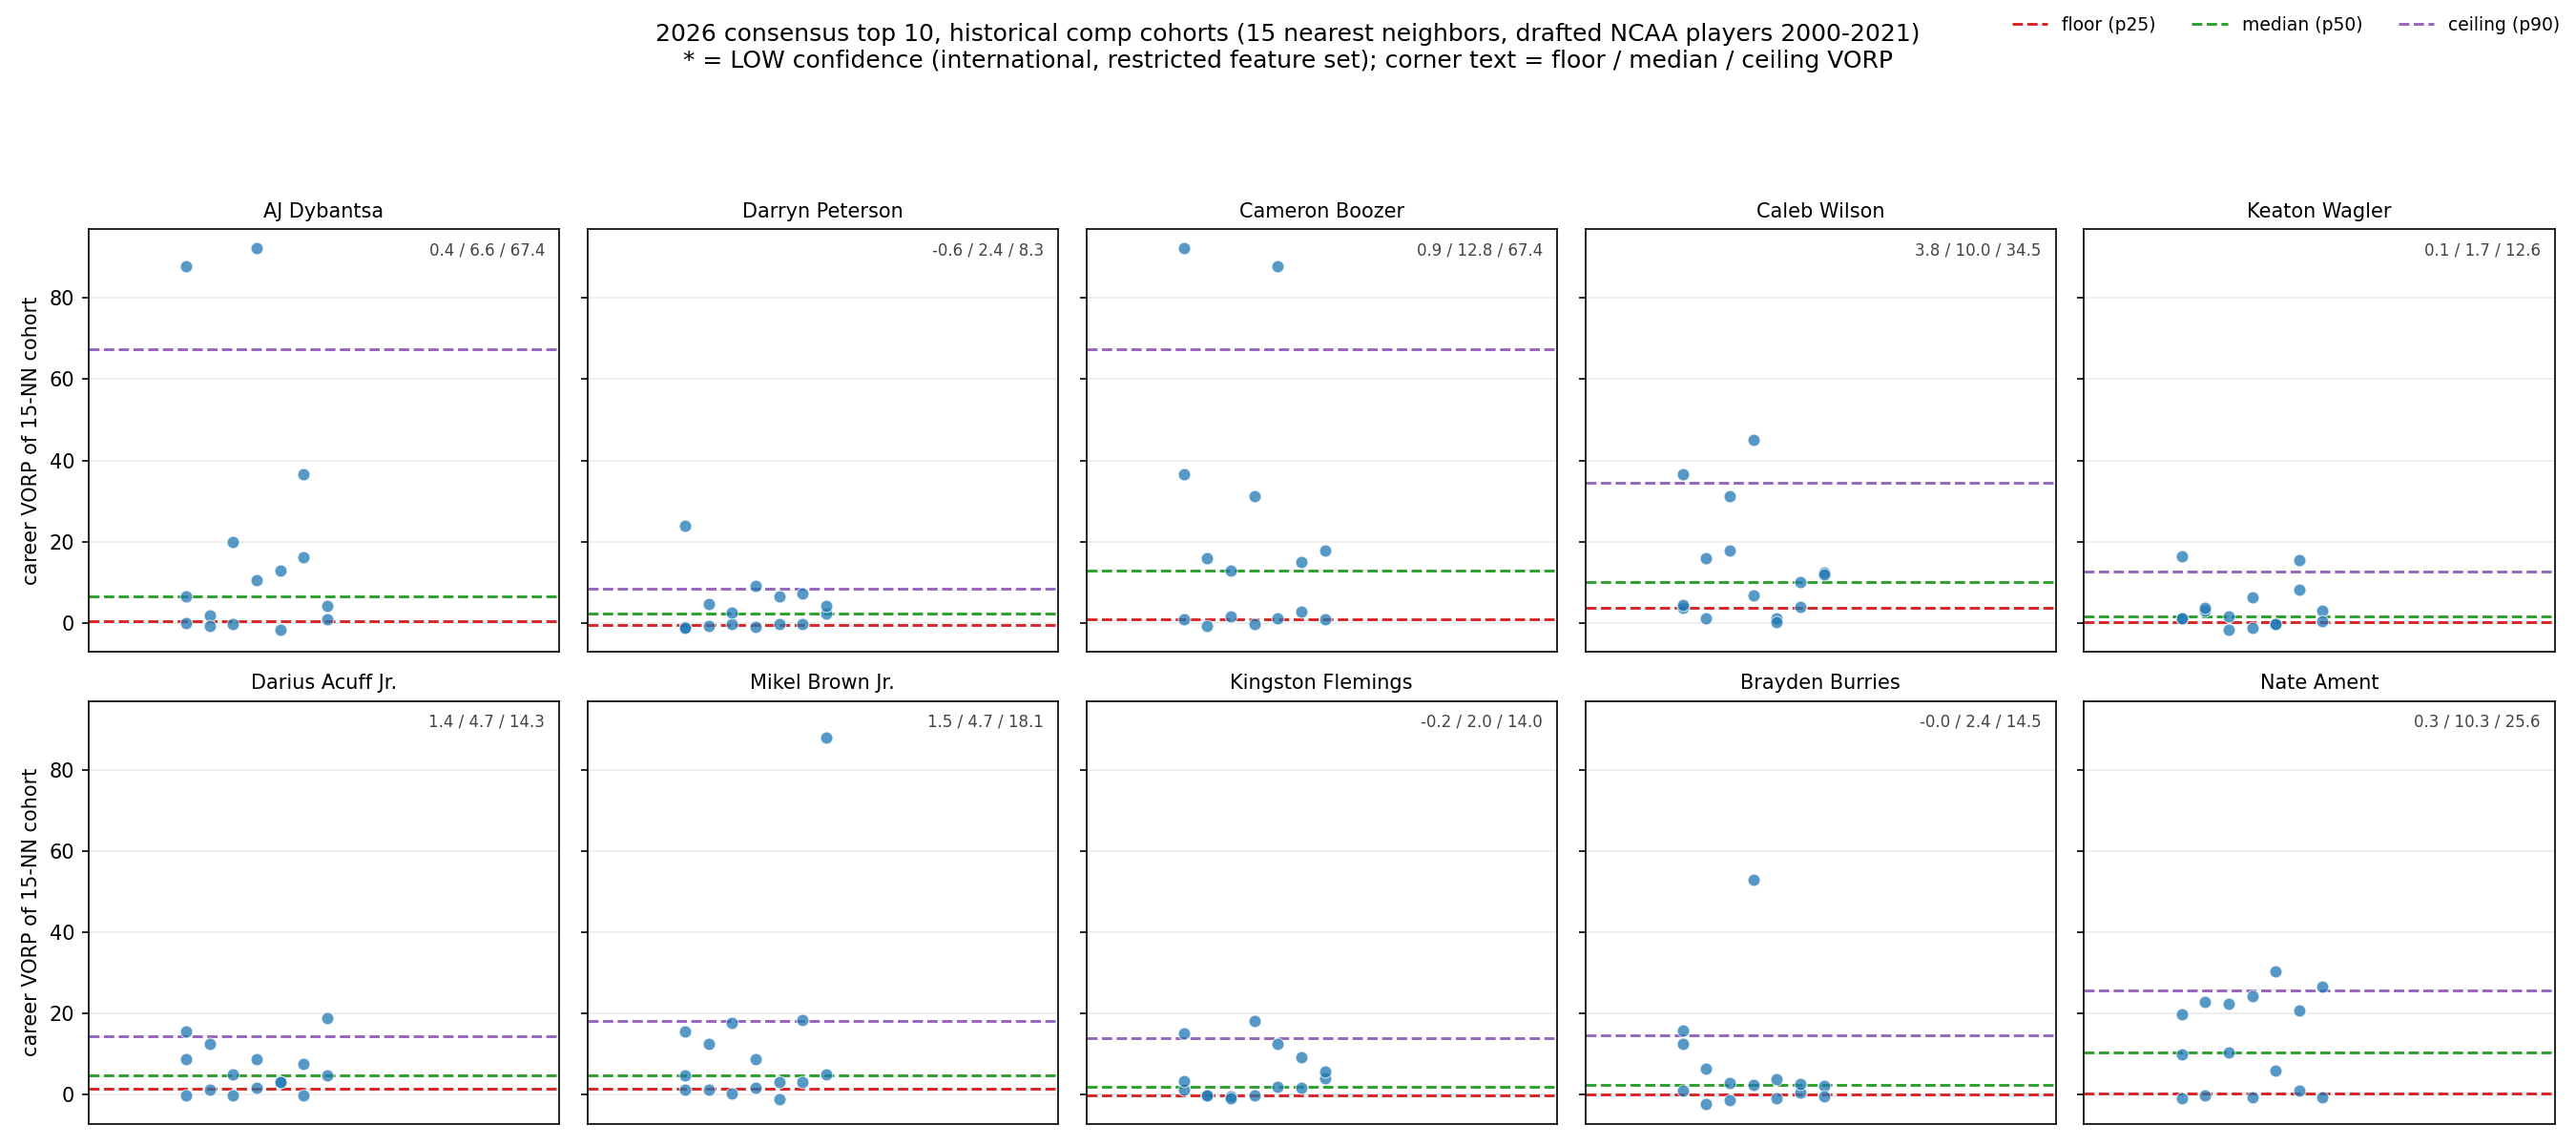
\includegraphics[keepaspectratio,alt={Comp-cohort career VORP distributions (floor / median / ceiling) for the top 10 board prospects, from the 781-player NCAA pool. Boozer's cohort carries the class's best All-Star rate (40\%); Peterson's is visibly suppressed by his 24-GP season.}]{../figures/comp_cohorts_top10.png}}
\caption{Comp-cohort career VORP distributions (floor / median / ceiling) for
the top 10 board prospects, from the 781-player NCAA pool. Boozer's cohort
carries the class's best All-Star rate (40\%); Peterson's is visibly suppressed
by his 24-GP season.}
\end{figure}

\subsection{D. VORP model coefficients and
importances}\label{d.-vorp-model-coefficients-and-importances}

Standardized coefficients (asinh-VORP target) and permutation importance, from
\texttt{models/metrics\_regression.json}. Ridge alpha 92.4, lasso alpha 0.0149
(both selected by inner CV). Lasso zeroes 6 of 21 features and keeps the same
leaders, confirming the feature story.

{\def\LTcaptype{none} % do not increment counter
\begin{longtable}[]{@{}llll@{}}
\toprule\noalign{}
Feature & Ridge coef (std) & Lasso coef (std) & Permutation importance \\
\midrule\noalign{}
\endhead
\bottomrule\noalign{}
\endlastfoot
age\_at\_draft & -0.380 & -0.390 & +0.0907 \\
height\_in & -0.030 & -0.003 & -0.0006 \\
weight\_lbs & -0.018 & -0.012 & -0.0003 \\
wingspan\_in & +0.025 & +0.000 & +0.0000 \\
standing\_reach\_in & +0.010 & +0.000 & +0.0000 \\
wing\_minus\_height & +0.027 & +0.032 & -0.0008 \\
ncaa\_ts\_pct & +0.052 & +0.015 & -0.0003 \\
ncaa\_usg\_pct & +0.029 & +0.022 & -0.0007 \\
ncaa\_ast\_pct & +0.099 & +0.071 & +0.0059 \\
ncaa\_tov\_pct & -0.011 & +0.000 & +0.0000 \\
ncaa\_stl\_pct & +0.032 & +0.001 & +0.0001 \\
ncaa\_blk\_pct & +0.039 & +0.000 & -0.0004 \\
ncaa\_ft\_pct & +0.035 & +0.025 & -0.0008 \\
ncaa\_3pa\_per40 & +0.013 & +0.000 & +0.0000 \\
ncaa\_obpm & -0.041 & -0.018 & -0.0006 \\
ncaa\_bpm & +0.355 & +0.388 & +0.0844 \\
miss\_age & -0.174 & -0.180 & +0.0503 \\
miss\_anthro & -0.014 & -0.000 & +0.0000 \\
miss\_wingspan & -0.050 & -0.045 & -0.0007 \\
miss\_ncaa\_core & -0.240 & -0.253 & +0.0395 \\
miss\_ncaa\_adv & +0.161 & +0.145 & +0.0023 \\
\end{longtable}
}

\subsection{E. Bust model calibration
bins}\label{e.-bust-model-calibration-bins}

From \texttt{models/metrics\_bust.json} (skill logistic, LODCO out-of-fold;
plotted in \texttt{figures/calibration\_bust.png}).

{\def\LTcaptype{none} % do not increment counter
\begin{longtable}[]{@{}ll@{}}
\toprule\noalign{}
Mean predicted bust probability & Observed bust fraction \\
\midrule\noalign{}
\endhead
\bottomrule\noalign{}
\endlastfoot
0.100 & 0.130 \\
0.167 & 0.122 \\
0.226 & 0.298 \\
0.281 & 0.275 \\
0.339 & 0.328 \\
0.411 & 0.385 \\
0.495 & 0.504 \\
0.586 & 0.573 \\
0.766 & 0.748 \\
0.995 & 1.000 \\
\end{longtable}
}

\subsection{F. Pointers}\label{f.-pointers}

\begin{itemize}
\tightlist
\item
  Full per-player dossiers (measurements, model drivers, comp cohorts, film
  notes, team fits): \texttt{dossiers/} (30 files plus
  \texttt{honorable\_mentions.md}).
\item
  Film notes with frame-tagged observations and cited scouting:
  \texttt{film/notes/} (20 prospects); report frames in
  \texttt{film/frames/\_report\_picks/}.
\item
  Machine-readable final board with per-player delta rationales:
  \texttt{data/processed/final\_board.csv}.
\item
  Per-slot team fit analysis: \texttt{data/processed/team\_fit.md}; mock:
  \texttt{data/processed/mock\_draft.csv}.
\item
  Model iteration log and tier definitions: \texttt{models/iterations.md},
  \texttt{models/tier\_definitions.md}.
\item
  Project chronology and incident log: \texttt{progress.md}. Full source log:
  \texttt{sources.md}.
\end{itemize}

\emph{All first-party film observations in this project are frame-based (1 fps
stills) and labeled as such; stills cannot show speed, burst, timing, or feel,
and no claim in this report pretends otherwise.}

\end{document}
